\documentclass[12pt,a4paper,titlepage]{article}
%\usepackage[doublespacing]{setspace}
\usepackage[utf8]{inputenc}         %This is used for ASKII digits.
\usepackage{amsmath, amssymb}       %This is for mathematic statements,check"amath.colorado.edu/documentation/LaTex/Symbols.pdf"
\usepackage{booktabs}
\usepackage{caption2}
\usepackage{epstopdf}
\usepackage{amsfonts,mathrsfs}      %fonts~~
\usepackage{graphicx}               %This is for graph inserting.
\usepackage{paralist}               %Give me compact lists!!!!! 'compactitem' 'compactenum' 'compactdesc'
%\usepackage{bm}                     %various kinds of bold texts.
\usepackage[top =2.54cm, bottom =2.54cm, left =3.18cm, right =3.18 cm]{geometry}
\usepackage{indentfirst}            %Indent the first letter
\usepackage{fancyhdr}               %Below is the head of the article.
\pagestyle{fancy}
\usepackage{lastpage}
\lhead{Team \# 33131}
\rhead{Page \thepage{} of \pageref{LastPage}}
\cfoot{}
%\numberwithin{equation}{section}    %Numbering of the equations will be based on sections.
%\usepackage{amsthm}
%\theoremstyle{definition}
%\newtheorem{def}{Definition}  %Below set the theorem system.
%\theoremstyle{plain}
%\newtheorem{thm}[law]{Thm}
%\theoremstyle{remark}
%\newtheorem*{remark}{Remark}
\newcommand{\boldit}[1]{\textbf{\textit{#1}}}
\renewcommand{\captionlabelfont}{\small \bfseries \rmfamily}
\usepackage{float}
\usepackage{paralist}
\usepackage{url}

\begin{document}

\title{Human Capital Model} \date{\today{}}
\maketitle

\tableofcontents

\newpage

\section{Introduction}
\label{sec:introduction}

\subsection{Restatement of the Problem}
\label{sec:restatement-of-the-problem}
We are required to build a mathematical model to solve the problem of heating water in bathtub. Thus we have some subproblems:
\begin{itemize}
\item Build a basic model that demonstrates the change of the temperature in the bathtub in space and time without other interventions.
\item Figure out the influence of parameters such as the shape of the bathtub or the motions made by the person or so.
\item Propose a strategy to keep the temperature as even as possible.
\end{itemize}
In the first step, we build the simplest model. The shape of the bathtub is a cuboid, and the person will stay still. In the second step, the person moves slowly and the shape of the bathtub changes. In the third step, we develop the conclusion of the strategy.

\section{Terminology}
\label{sec:terminology}

Definitions of symbols employed in this paper are listed in Table \ref{1_t} and Table \ref{2_t}.
\begin{table}
\begin{tabular}{l|l}
  Constant & Description \\
  \hline
  $k$            &Thermal conductivity of water \\
  $\rho$         &Density of water \\
  ${\rho}_a$     &Density of air \\
  ${\gamma}_1$   &Heat exchange coefficient between water and air \\
  ${\gamma}_2$   &Heat exchange coefficient between water and person \\
  ${\gamma}_3$   &Heat exchange coefficient between water and bathtub \\
  $C_w$          &Specific heat capacity of water \\
  $C_a$          &Specific heat capacity of air \\
  $V$            &Total volume of water \\
  $V_a$          &Total volume of air above the water \\
  $v$            &Flow velocity of air\\
  $x_s$          &Humidity ratio in saturated air \\
  $x$            &Humidity ratio in the air \\
  $x_0$          &Initial humidity ratio in the air \\
  $A$            &Square of water surface \\
  $V_a$          &Volume of surrounding air \\
  $C_v$          &Evaporation heat of water \\
\end{tabular}
\caption{Constant}\label{1_t}
\end{table}


\begin{table}
\begin{tabular}{l|l}
  Variable & Description \\
  \hline
  $t$            &time \\
  $u$            &Temperature of water \\
  $u$            &Temperature of water when t=0 \\
  $u_1$          &Temperature of air \\
  $u_2$          &Temperature of person's surface \\
  $u_3$          &Temperature of bathtub \\
  $u_h$          &Temperature of hot water from faucet \\
  $v_h$          &Velocity of hot water from faucet \\
  $g$            &Evaporation heat of water\\
\end{tabular}
\caption{Variable}\label{2_t}
\end{table}

\section{Assumptions and Justifications}
\label{sec:assumptions-and-justifications}

\begin{itemize}
\item \textbf{assumption 1} If an employee has probability to
  promote, he won't churn.

The possibility of the unforeseen accidents, which could force an
employee to leave his position,is neglected.Human nature, an employee
will stay at his position to chase for higher level.

\item \textbf{assumption 2} For a vacancy,if there exists an
  employee measures up to it already,ICM won't recruit for it.

Since recruiting good people is difficult, time consuming and
expensive according to issue 5,it is wasteful to recruit for a
position if an employee can promote to it.

\item \textbf{assumption 3} Demotion won't occur.

\item \textbf{assumption 4} Administrative clerk won't promote or be
  transferred.

\item \textbf{assumption 5} For the promotion probability and
  organization change, the other factors effects the churn probability
  is invariable.

Though churn derives from varieties of reasons and they are actually
lacking of known conditions and data to estimate them, we have to
regard it as stable in our model.

\item \textbf{assumption 6} Each division or office have at least one
  middle manager or senior manager.

\end{itemize}

% the main section of the paper
\section{Water in the Bathtub Model}
\label{sec:human-capital-model}


\subsection{Model Overview}
\label{sec:model-overview}

Partial differential equations are widely used in natural science, engineering and economical management.
It is natural to use partial differential equation to solve this physical problem.

In our model, five factors account for heat transfer of water: heat exchange between water and air, heat
exchange between water and the person, heat exchange between water and the bathtub, heat energy of hot water from the
faucet and heat energy of water flow outside. According to thermology, we deduce the equation
of water temperature in the bathtub. The initial-boundary value conditions are deduced according to
Fourier theorem, vaporization equation\cite{1}.

Since the equation is a relatively complex 3D partial differential equation, we use matlab to solve it.
We build a geometry as the bathtub. By finite element method, the geometry is divided into several parts.
The solution of each part is considered to be a relatively precise value solution.



\subsection{Heat Equation}
\label{sec:heat equation}

In this part, we use physical theorem to deduce the heat conduction equation in the bathtub.

Figure \ref{1_p} shows thermal analysis of water in bathtub.
\begin{figure}[htb]
  \centering
  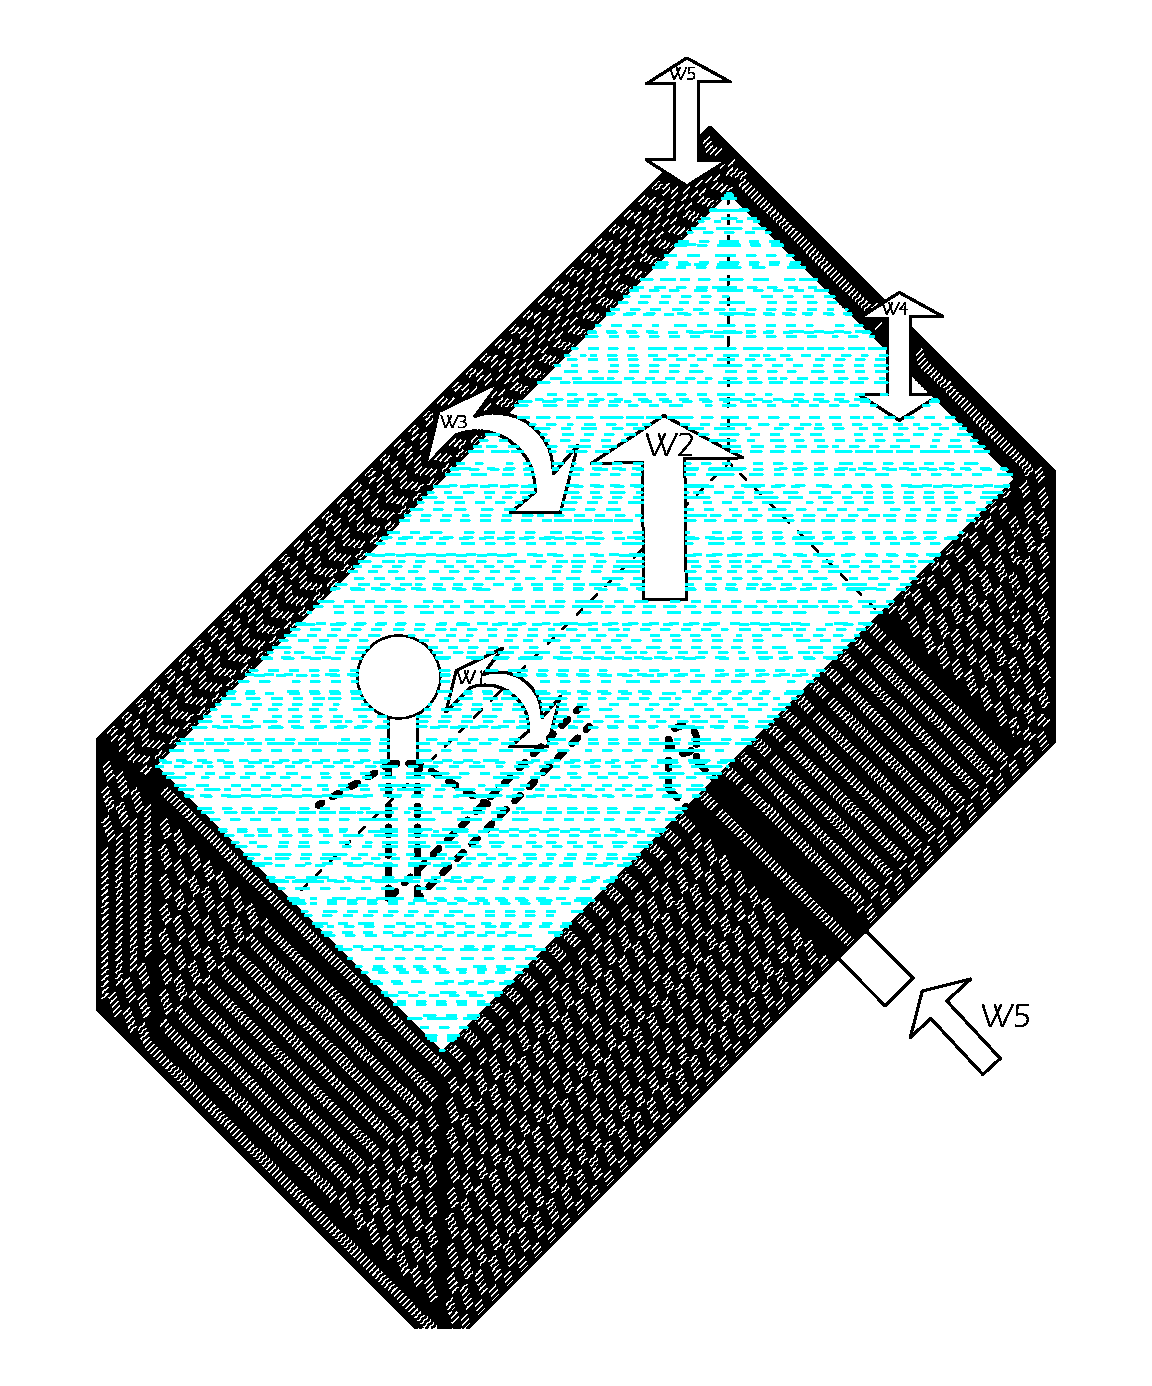
\includegraphics[width=8cm]{2.pdf}\\
  \caption{Thermal Analysis of Water}\label{1_p}
\end{figure}

First, we assume that the heat change of all the water in a tiny time $\Delta t$ from $t_1$ to $t_2$ is $\Delta Q$.
As shown in Figure 1, heat of water in the bathtub exchanges with air, the person and the bathtub.
In addition, heat changes when the hot water flows in and the excess water flows out.
Thus $\Delta Q$ is divided into five parts, i.e.
\begin{equation}
 \Delta Q=\Delta Q_1+\Delta Q_2-\Delta Q_3-\Delta Q_4
\end{equation}
in which $\Delta Q_1$ is the heat transferred from air, person and bathtub,
$\Delta Q_2$ is the heat of the hot water from the faucet in $\Delta t$,
$\Delta Q_3$ is the heat of the water flows away in $\Delta t$,
$\Delta Q_4$ is the heat loss because of vaporization.

Totally, internal energy of water changes when heat exchanges happen.
Then the temperature changes according to the equation
\begin{equation}
 Q=\iiint\limits_{\Omega}\rho C_{w}(u_f - u_i)dx dy dz
\end{equation}
in which $\Omega$ is the region of water, $\rho$ represents the density of water, $u_f$ stands for the final temperature when t=$t_2$, and $u_i$ is the initial temperature when t=$t_1$.

Considering the right side of equation 1,
 Fourier theorem indicates that,
\begin{equation}
 dQ=-k\frac{\partial u}{\partial n}dSdt
\end{equation}
holds for the heat flows through surface with square of dS, as it shows in Figure \ref{2_p}.
\begin{figure}[htb]
  \centering
  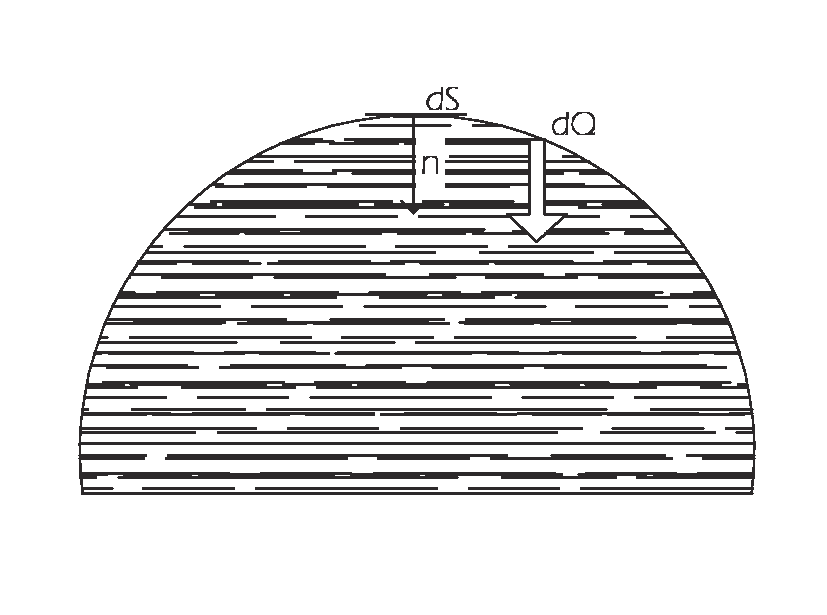
\includegraphics[width=8cm]{1.pdf}\\
  \caption{Thermal Analysis}\label{2_p}
\end{figure}
In the equation, k is thermal conductivity, $\frac{\partial u}{\partial n}$ is the derivative of u along the normal line. Thus, after integration of dQ by time and space
\begin{equation}
 \Delta Q_1=\int_{t_1}^{t_2}[{\int_{\Gamma}}k\frac{\partial u}{\partial n}dS]dt
\end{equation}
in which $\Gamma$ is the boundary of $\Omega$,
the heat flows into the water by thermal conduction could be calculated.

$\Delta Q_2$ is determined by the internal energy of hot water from the faucet in $\Delta t$.
And $\Delta Q_2$ can be calculated by
$\Delta Q_2={\Delta m}C{u_h}$.
Since the hot water is constant,
$\Delta m=v{\Delta t}$.

It is obvious that the excess water is the same value of hot water in any time period.
Thus $\Delta Q_3$ can be calculated by
$\Delta Q_3={\Delta m}{C_w}u$.
Also, $\Delta m=v{\Delta t}$.
$\Delta v$ is the weight of hot water per second, $\Delta m$ is the weight of hot water flows in during $\Delta t$.

According to thermal theorem, heat loss in vaporization is proportional to the weight of vapor water.
$\Delta Q_4={C_v}\Delta {m_v}$.
$\Delta {m_v}$ is the weight of evaporation water in $\Delta t$, ${C_v}$ is evaporation heat of water per kilogram.

Since water could be considered as manifold, according to Green formula, we deduce the formula
\begin{displaymath}
\begin{aligned}
\int_{t_1}^{t_2} \iint\limits_{\Gamma}k\frac{\partial u}{\partial n}dsdt & =\iiint\limits_{\Omega}\rho C_{w}(u_f - u_i)dx dy dz\\
& =\int_{t_1}^{t_2}\iiint\limits_{\Omega}[\frac{\partial}{\partial x}(k\frac{\partial u}{\partial x})+\frac{\partial}{\partial y}(k\frac{\partial u}{\partial y})+\frac{\partial}{\partial z}(k\frac{\partial u}{\partial z})]dxdydx\\
& = \iiint\limits_{\Omega}\rho C_{w}(\int_{t_1}^{t_2}\frac{\partial u}{\partial t}dt)dxdydz
\end{aligned}
\end{displaymath}

Combining the equations above, we conclude that
\begin{equation}
\rho C_{w}\frac{\partial u}{\partial t}=k\bigtriangleup u+\frac{C_w V_h(u_h-u)}{V}-\frac{C_v g}{V}%
\end{equation}
In this heat equation, $u_h$ and $v_h$ are two variables that control the strategy.

Now let's discuss g, evaporation rate per square.
As Figure \ref{3_p} shows, water evaporates into air and air humidity increases, until it is saturate. According to empirical formula\cite{1}, we know that
\begin{equation}
 g=\frac{(25+19v)({x_s}-x)}{3600}
\end{equation}
in which v is the velocity of air, ${x_s}$ is humidity ratio in saturated air, $x$ is unsaturated humidity ratio in air.
Considering the humidity ratio in the air, it indicates
\begin{equation}
 x=x_0+\int \frac{Ag}{\rho V_a}dt
\end{equation}
in which $x_0$ is the initial humidity ratio in the air, $\rho$ is the density of water, $V_a$ is the total volume of surrounding air.
\begin{figure}[htb]
  \centering
  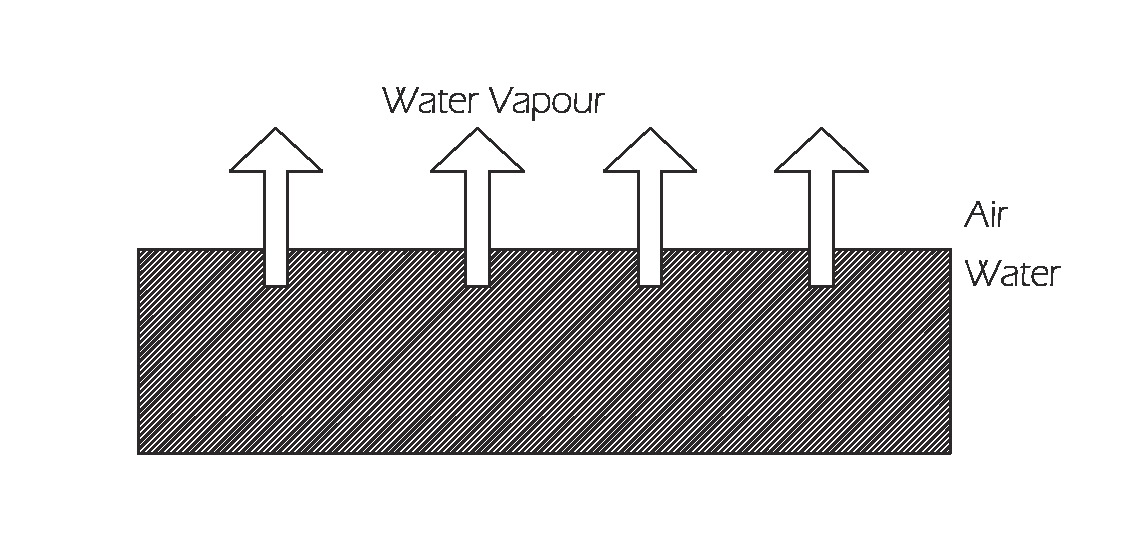
\includegraphics[width=8cm]{3.pdf}\\
  \caption{Evaporation}\label{3_p}
\end{figure}

Combing and differentiating two equations, we get an ordinary partial equation
\begin{equation}
 \frac{3600}{25+19v} \frac{dg}{dt}=\frac{A}{\rho {V_a}}
\end{equation}
Solving the equation, we get the solution
\begin{equation}
 g=\frac{(25+19v)({x_s}-{x_0})}{3600}e^{-\lambda t}, \lambda =\frac{A(25+19v)}{3600\rho {V_a}}
\end{equation}


\subsection{Initial-Boundary Value Condition}
\label{initial-boundary value condition}

Boundary value conditions are quite essential in partial differential equations. In our model, water is not a regular object. Thus boundary value condition is complex.

The boundary of water consists of four parts: water-air boundary, water-person boundary, water-bathtub boundary, and the square for faucet. We denote them as
${\Gamma}_1$, ${\Gamma}_2$, ${\Gamma}_3$, ${\Gamma}_4$ respectively.

Since bather is temperature-constant, the boundary value condition of ${\Gamma}_1$ and ${\Gamma}_3$ could be considered
as the Dirichlet value condition. That is
\begin{equation}
 u=u_i, (x,y,z)\in {\Gamma}_i, i=2.4
\end{equation}
In the equation, $u_2$ is the surface temperature of the person. We assume it is constant. $u_4$ is the temperature of hot water.

The boundary value condition of ${\Gamma}_1$ and ${\Gamma}_3$ could be considered as the third boundary value condition approximately. That is
\begin{equation}
 k\frac{\partial u}{\partial n}+{{\gamma}_i}u={{\gamma}_i}{u_i}, (x,y,z)\in {\Gamma}_i
\end{equation}
In the equation, i=1 or 3 ,$u_i$ is the temperature of contact material, and 
${\gamma}_i$ is the heat exchange coefficient of ${\Gamma}_i$.

In the equation above, $u_3$ is temperature of bathtub, we assume it is unchangeable and as same as initial air temperature.

$u_1$, the temperature of air, is time-dependant, because water vapor transfer heat to air. We can calculate $u_1$ by calculating the energy of water vapor evaporating in the air. Referencing the deduction of evaporation in the last section,
\begin{equation}
  u_1=u_0+\frac{C_w\rho}{C_a{{\rho}_a}} (x_s-x_0)(1-e^{-\lambda t})
\end{equation}

Consider the temperature of air, $u_1$. Heat exchange of air consists of two ways, heat conduction and evaporation.

In our model, we assume the temperature of water is equilibrium throughout the bathtub initially.

\subsection{PDE Solution}
\label{sec:PDE solution}
Since our equations are complex and the region is quite irregular, it's impossible to get a analytical solution. Finite element method is normally adopted to deal with this kind of problem.

We use Partial Differential Equation Toolbox in matlab to solve our equations. Partial Differential Equation Toolbox makes use of finite element method to separate irregular geometry, calculate a relatively precise solution, and get solution of temperature corresponding to different $u_h$ and $v_h$. By comparing temperature distributions, we choose proper parameters as the best strategy.

First, we build a 3D geometry model to simulate a proper-size bathtub, as it shown in Figure \ref{4_p}. Matlab divides the geometry into several elements.
\begin{figure}[htb]
  \centering
  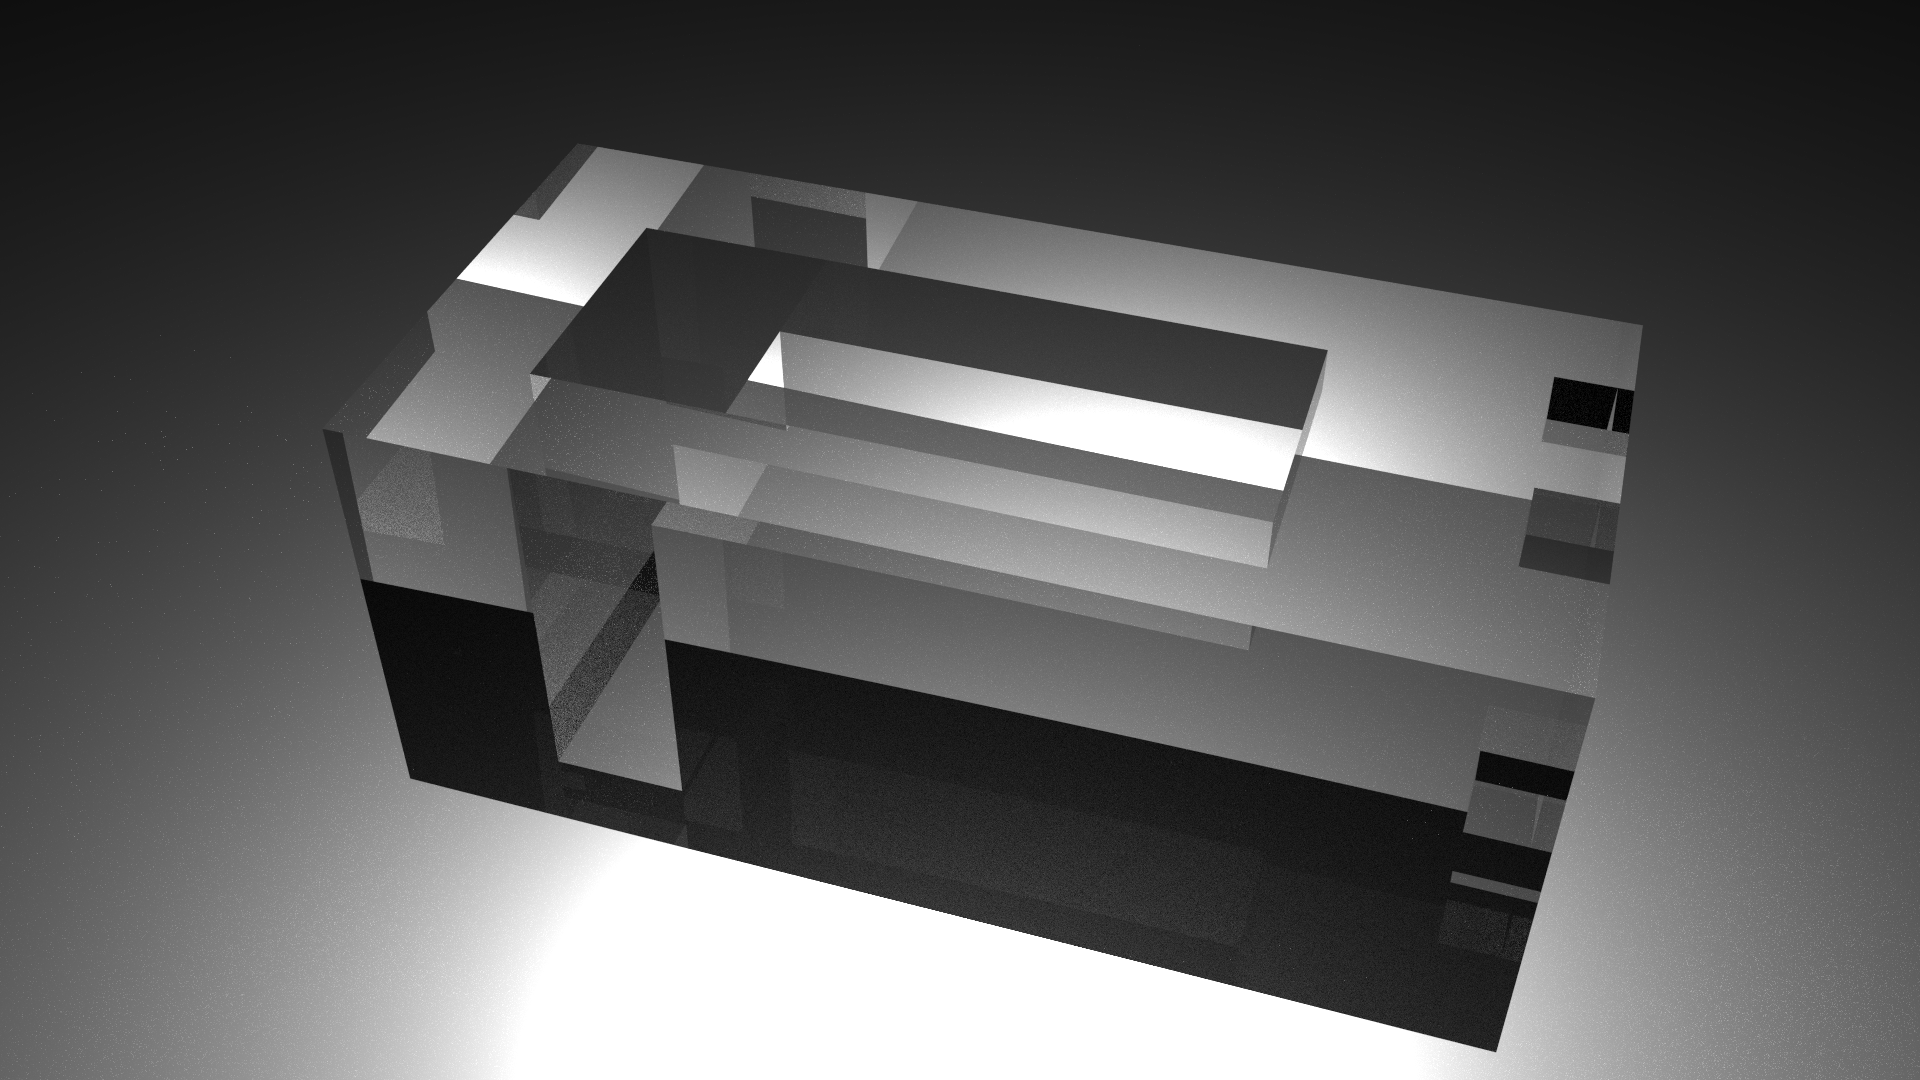
\includegraphics[width=8cm]{4.png}\\
  \caption{3D geometry of water}\label{4_p}
\end{figure}

Then we input the heat equation and initial-boundary value conditions. Boundary value conditions are different in three parts.

\section{Results and Analysis}
\label{sec:performance-and-analysis}

Our strategy focus on two variables, $v_h$ and $u_h$. We test about fifty pairs of data to find the best strategy. And we list nine representative pairs of data in Table \ref{3_t}.

\begin{table}
\begin{center}
\begin{tabular}{c|c}
\hline
    $v_h kg/s$  &${u_h}\,^{\circ}\mathrm{C}$        \\ \hline
     0.1             & 50              \\ \hline
    0.2             & 50              \\ \hline
     0.3             & 50              \\ \hline
     0.1             & 40              \\ \hline
     0.2             & 40              \\ \hline
     0.3             & 40              \\ \hline
     0.1             & 30              \\ \hline
     0.2             & 30              \\ \hline
     0.3             & 30              \\ \hline
\end{tabular}
\end{center}
\caption{Represenative Data Pairs}\label{3_t}
\end{table}

In each operation, $u_2$ is taken as $33.5\,^{\circ}\mathrm{C}$
and the initial value condition is $35\,^{\circ}\mathrm{C}$.
 We take 120s as time period. The following graphs show the results we get.

Figure \ref{5_p}, Figure \ref{6_p}, Figure \ref{7_p} show the temperature of water at t=240, with $u_h=40$ and $v_h=0.1, 0.2 and 0.3$
\begin{figure}[htb]
  \centering
  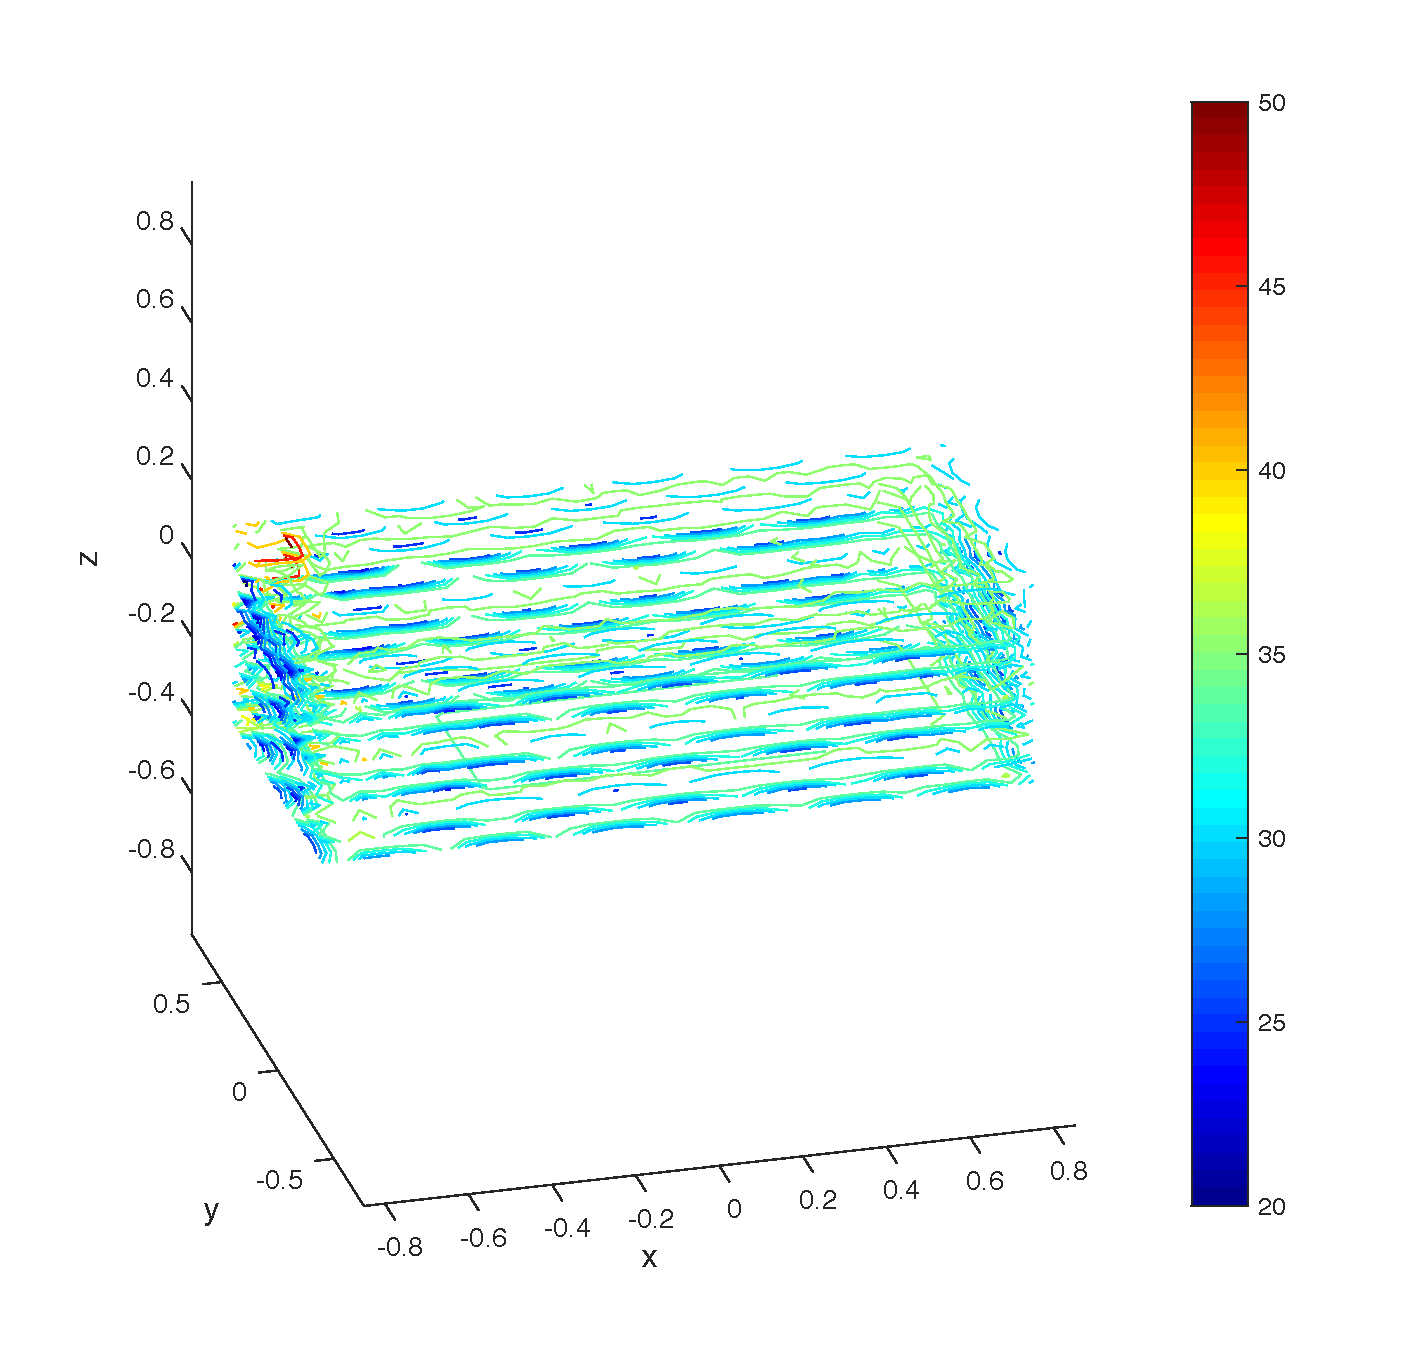
\includegraphics[width=8cm]{6-2.pdf}\\
  \caption{$u_h=40$, $v_h=0.1$, t=240}\label{5_p}
\end{figure}

\begin{figure}[htb]
  \centering
  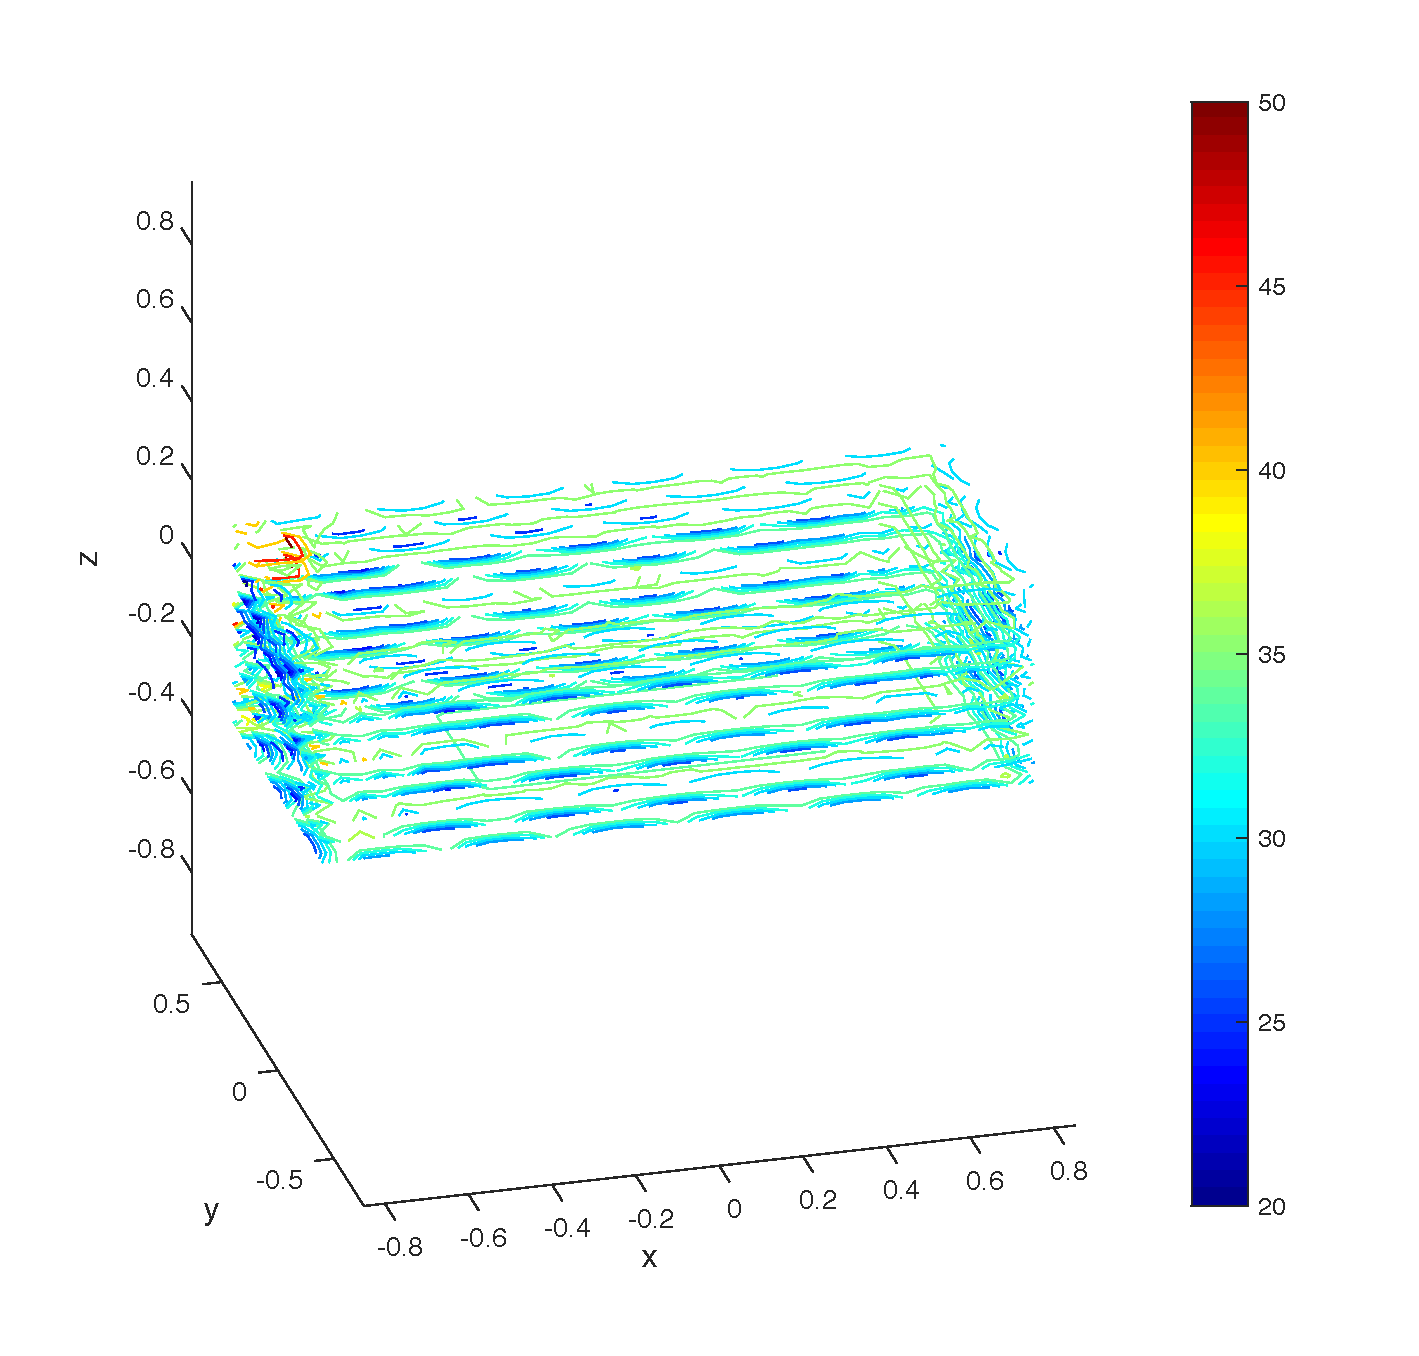
\includegraphics[width=8cm]{10-2.pdf}\\
  \caption{$u_h=40$, $v_h=0.2$, t=240}\label{6_p}
\end{figure}

\begin{figure}[htb]
  \centering
  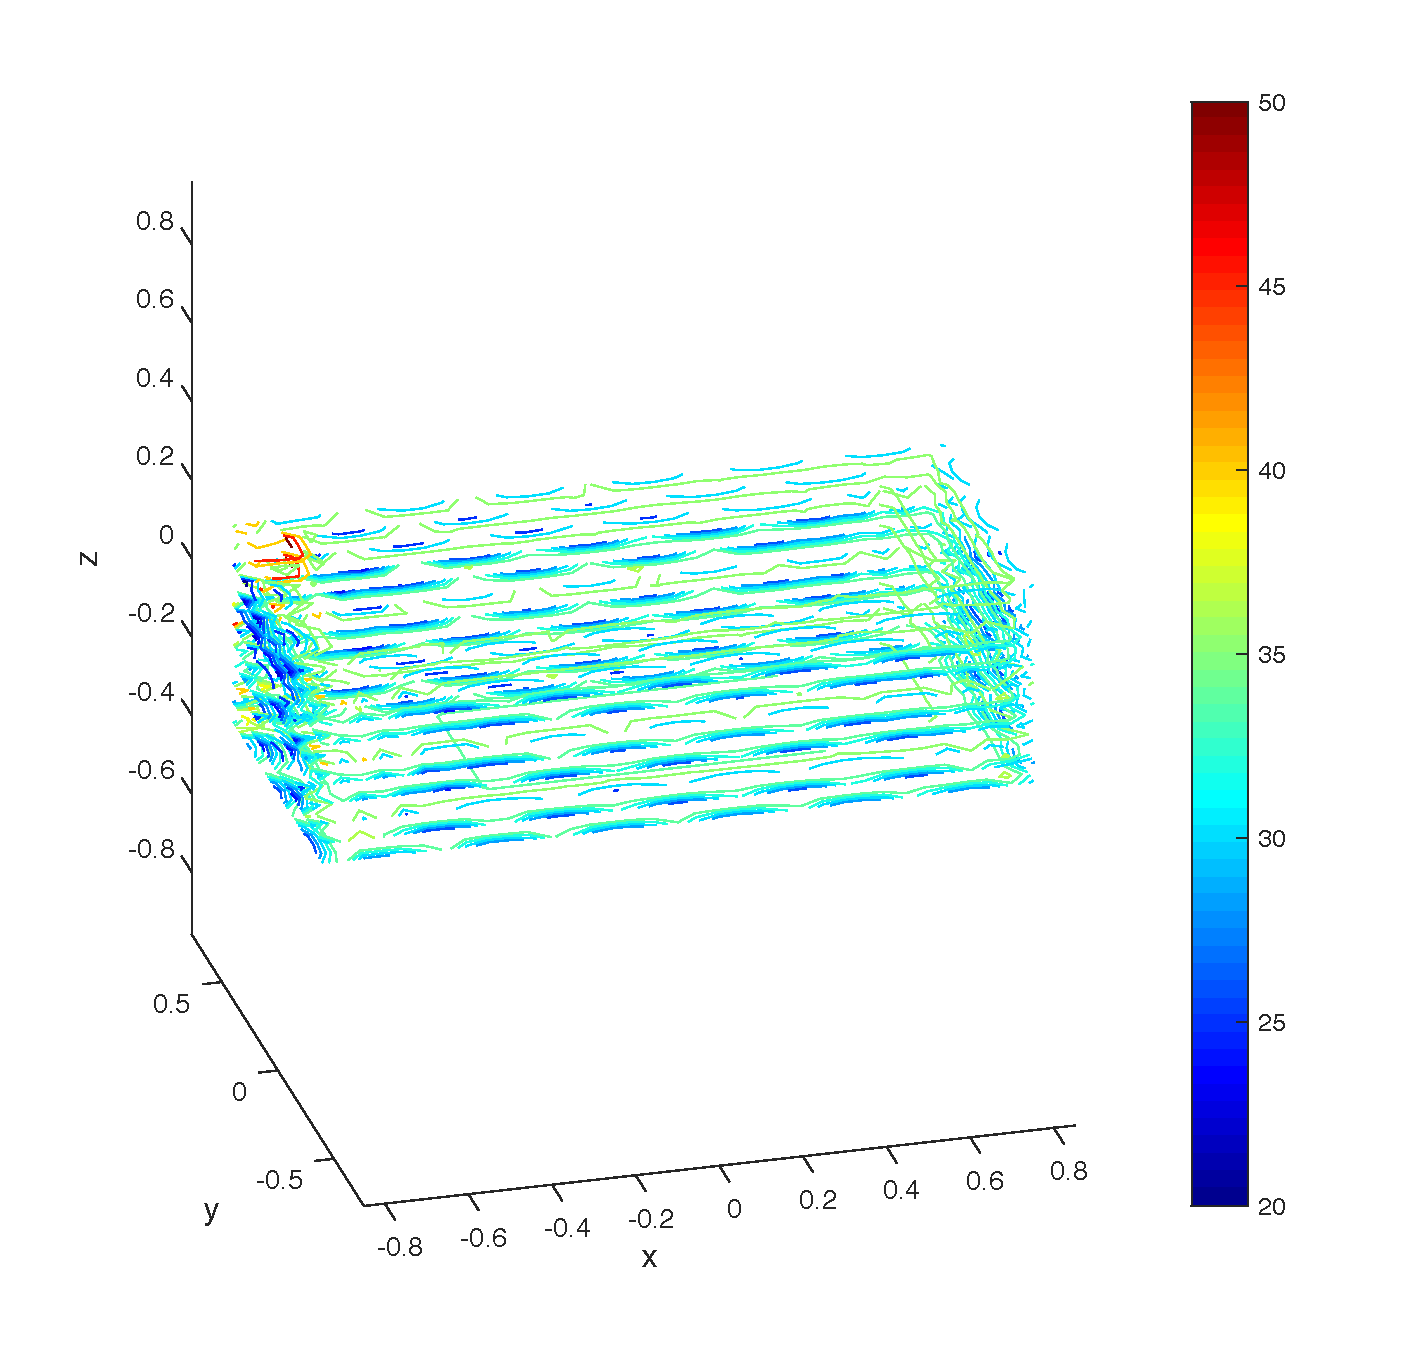
\includegraphics[width=8cm]{11-2.pdf}\\
  \caption{$u_h=40$,$v_h=0.3$,t=240}\label{7_p}
\end{figure}

Figure 8, Figure 9, Figure 10 show the temperature at t=600
\begin{figure}[htb]
  \centering
  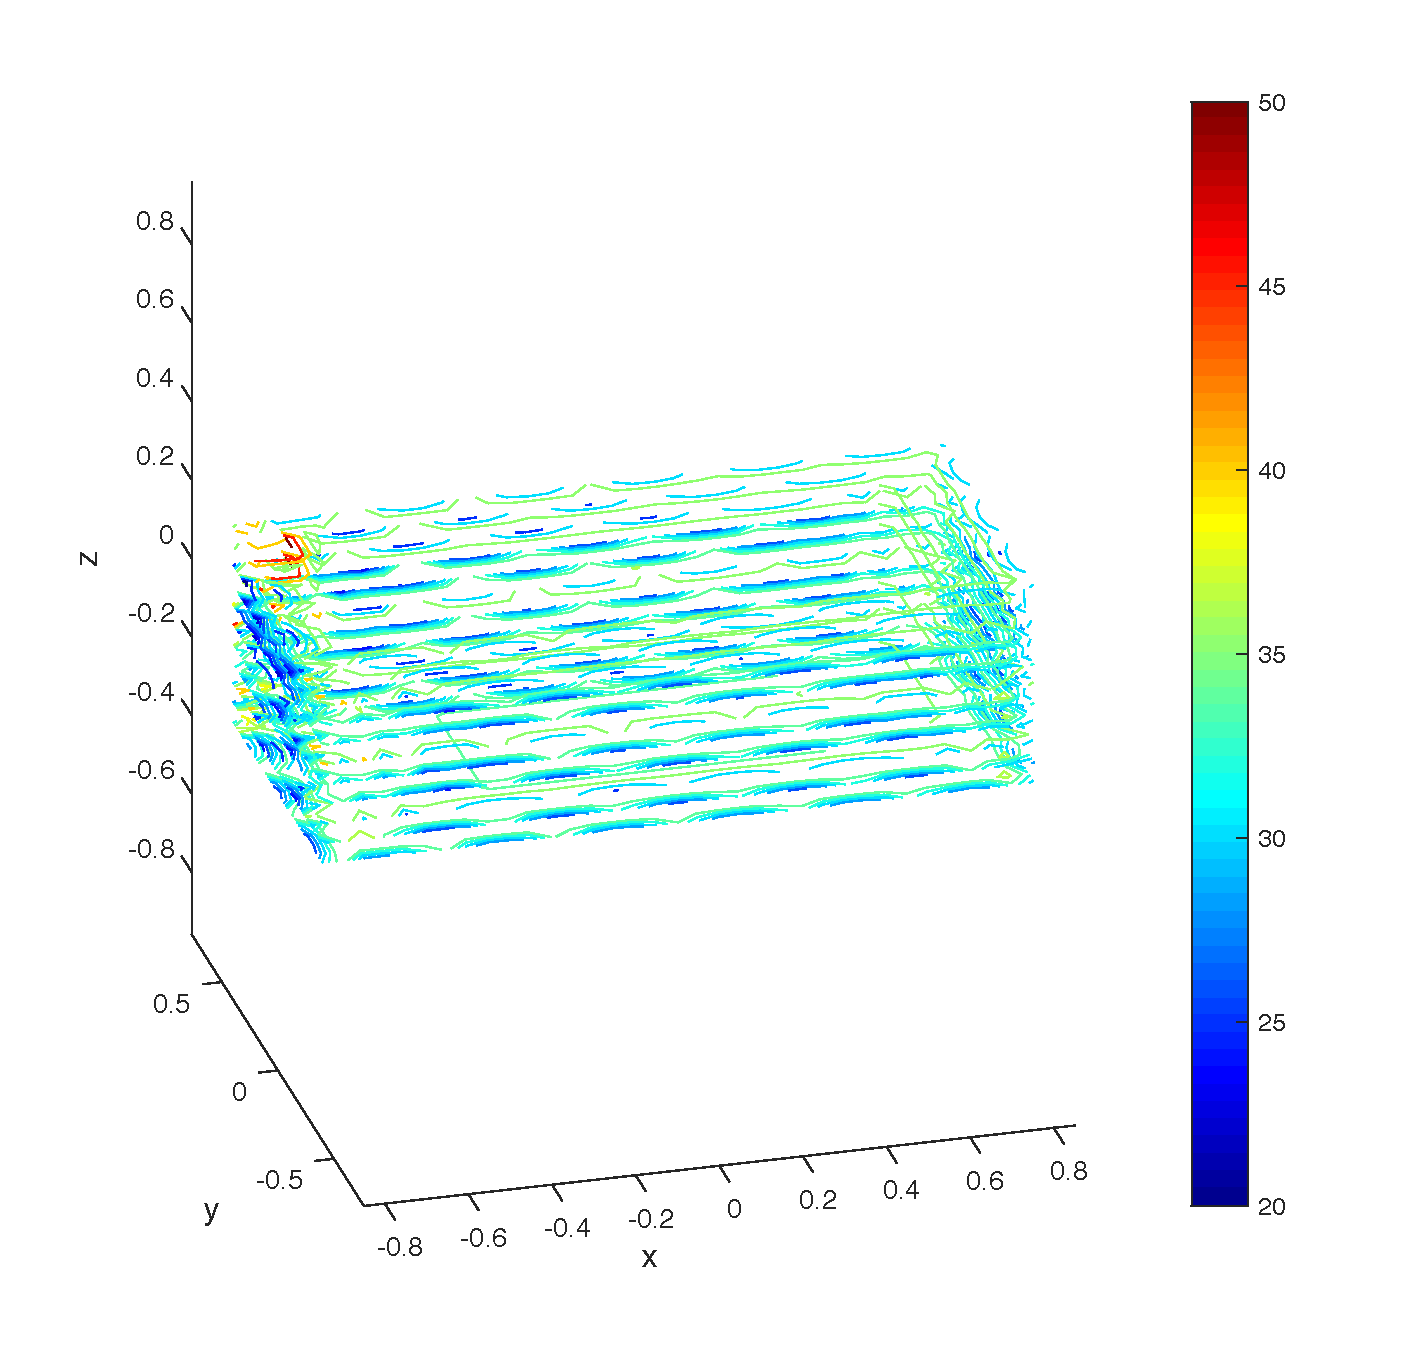
\includegraphics[width=8cm]{6-5.pdf}\\
  \caption{$u_h=40$,$v_h=0.1$,t=600}\label{6-5_p}
\end{figure}

\begin{figure}[htb]
  \centering
  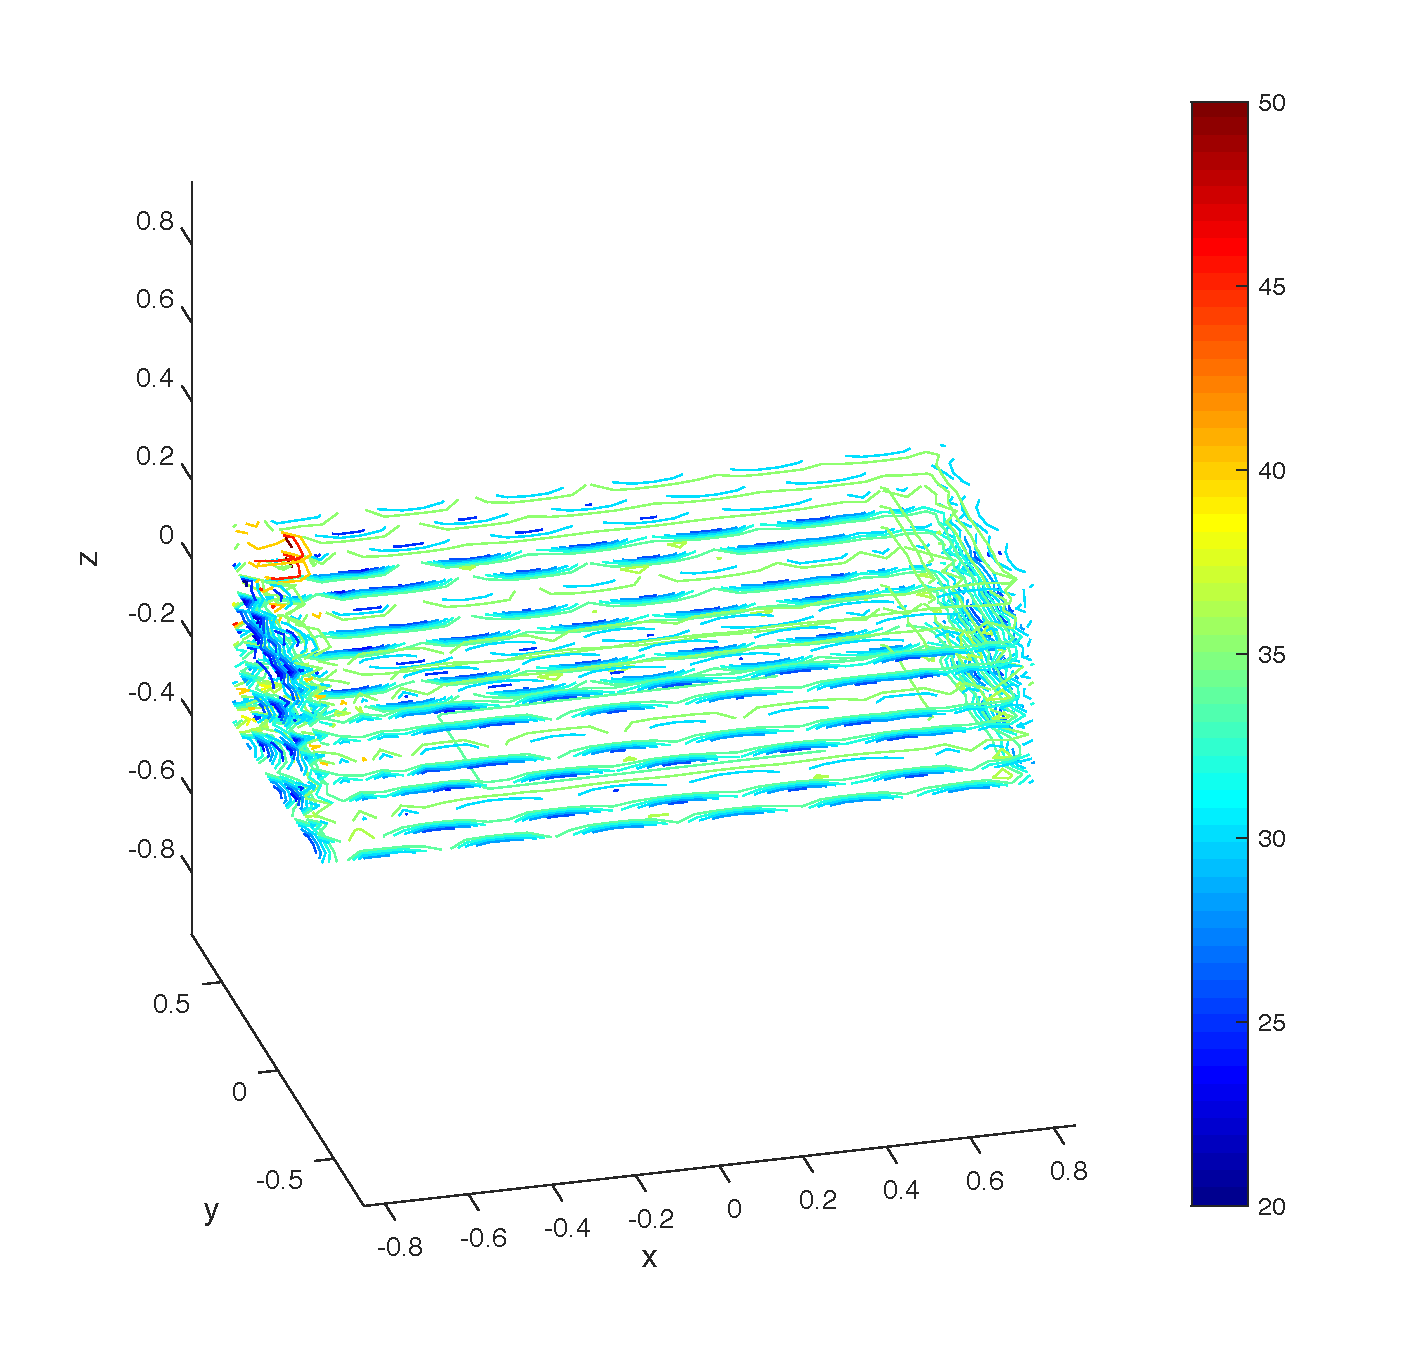
\includegraphics[width=8cm]{10-5.pdf}\\
  \caption{$u_h=40$,$v_h=0.2$,t=240}\label{10-5_p}
\end{figure}

\begin{figure}[htb]
  \centering
  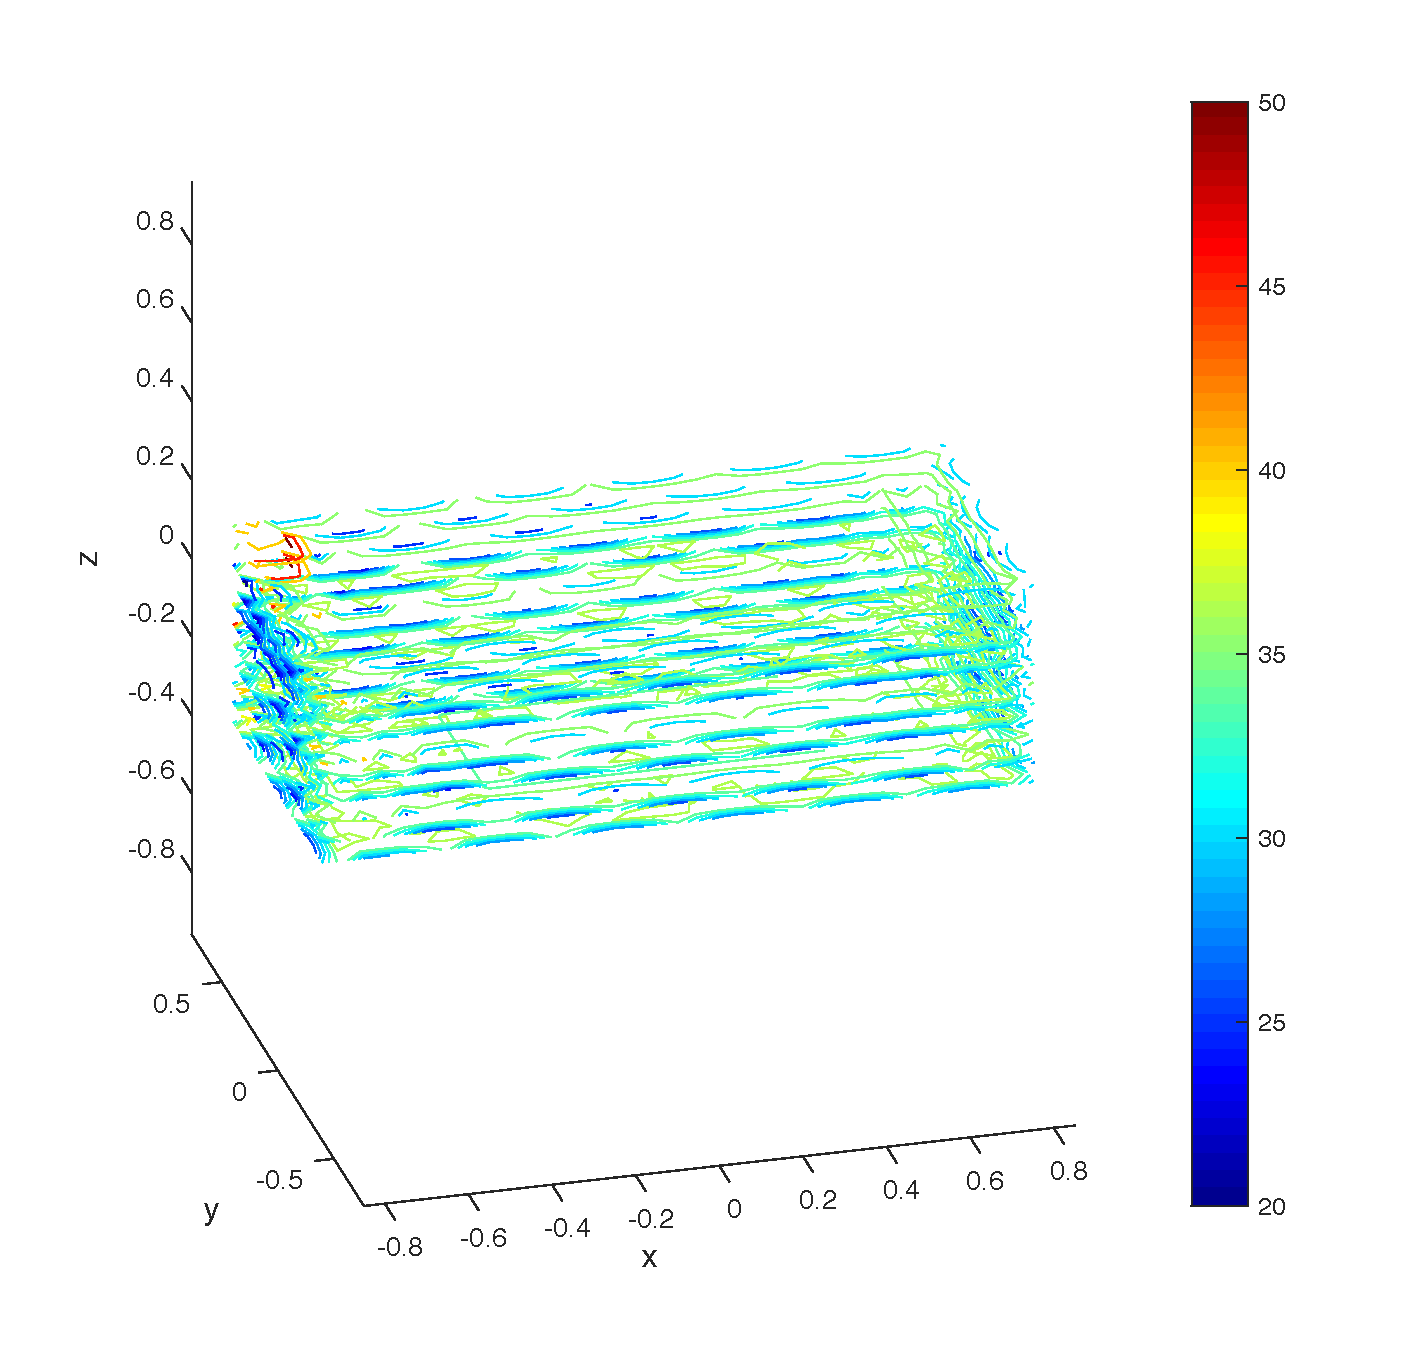
\includegraphics[width=8cm]{11-5.pdf}\\
  \caption{$u_h=40$,$v_h=0.3$,t=600}\label{11-5_p}
\end{figure}

It indicates that keep $u_h$, temperature increases when $v_h$ increases, and the system becomes more stable as time goes on. It proves that our model is sensible.

  
Figure 11, Figure 12, Figure 13 show the temperature of water at t=240, with $v_h=0.2$ and $u_h=30, 40 and 50$

\begin{figure}[htb]
  \centering
  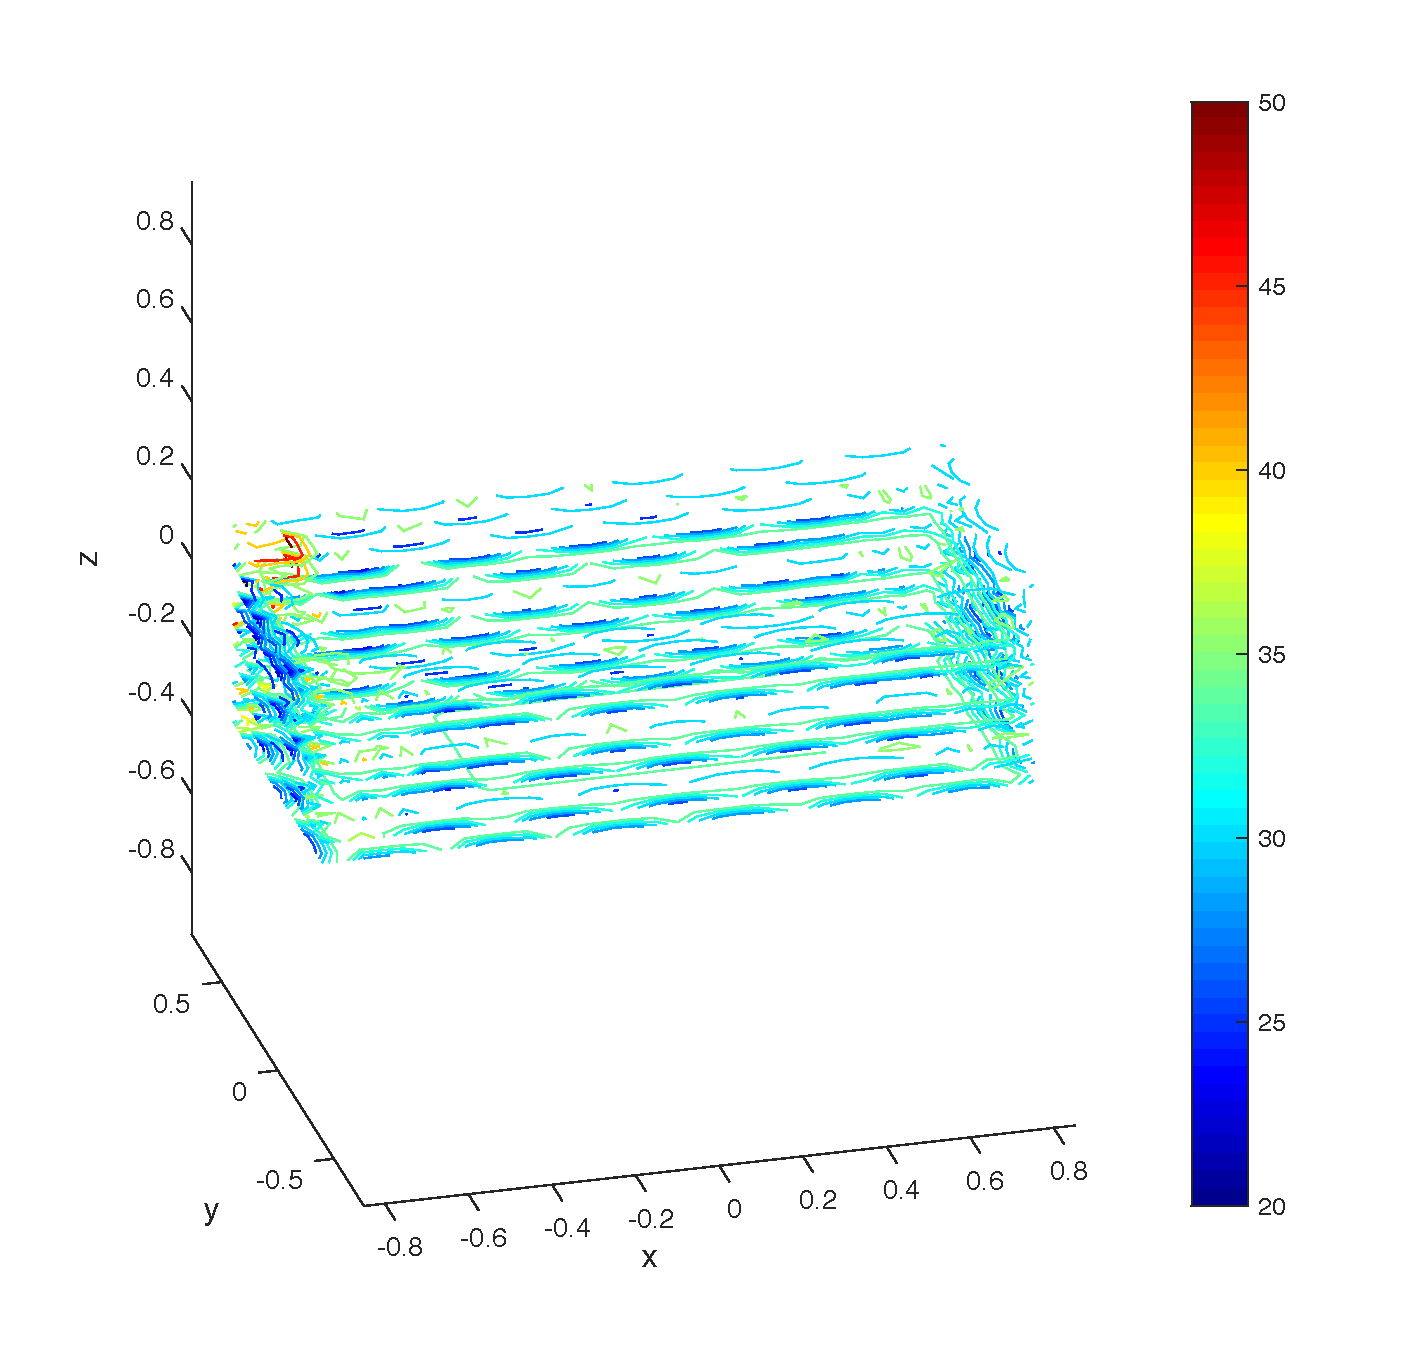
\includegraphics[width=8cm]{8-2.pdf}\\
  \caption{$u_h=30$,$v_h=0.2$,t=240}\label{8-2_p}
\end{figure}

\begin{figure}[htb]
  \centering
  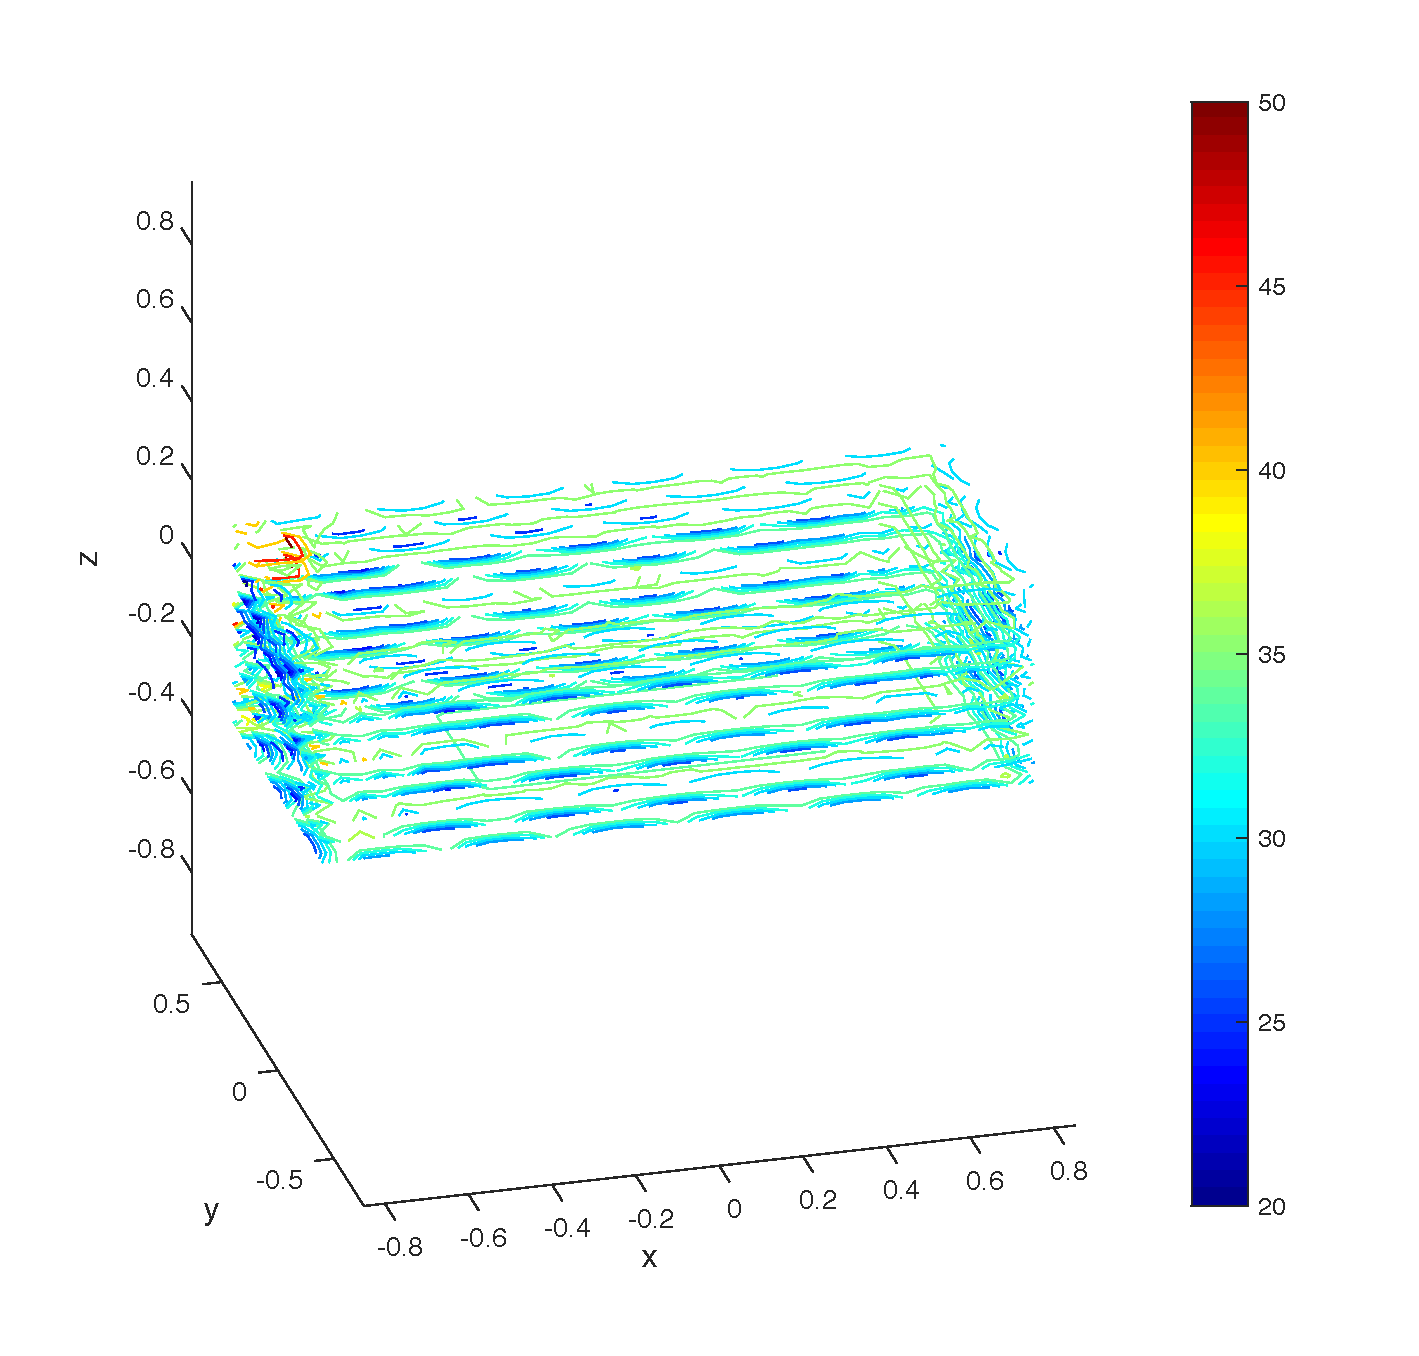
\includegraphics[width=8cm]{10-2.pdf}\\
  \caption{$u_h=40$,$v_h=0.2$,t=240}\label{10-2_p}
\end{figure}

\begin{figure}[htb]
  \centering
  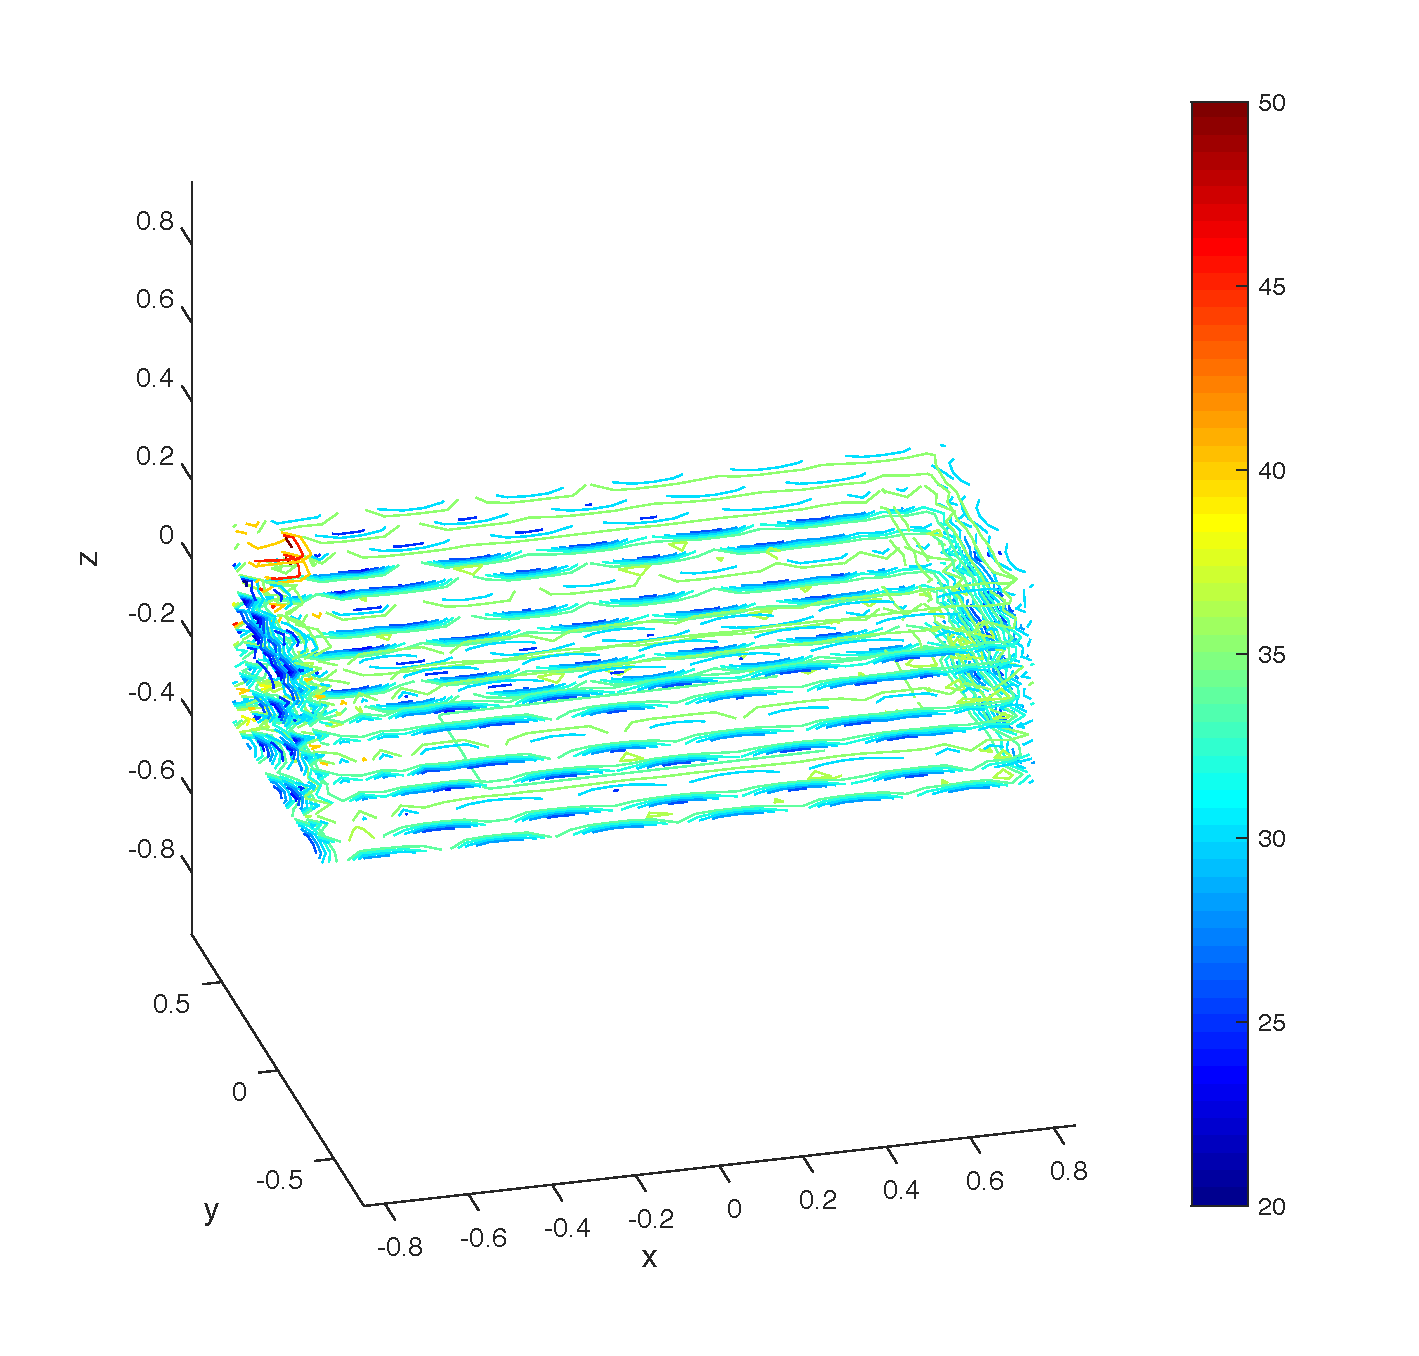
\includegraphics[width=8cm]{4-2.pdf}\\
  \caption{$u_h=50$,$v_h=0.2$,t=240}\label{4-2_p}
\end{figure}

Figure 14, Figure 15, Figure 16 show the temperature at t=600

\begin{figure}[htb]
  \centering
  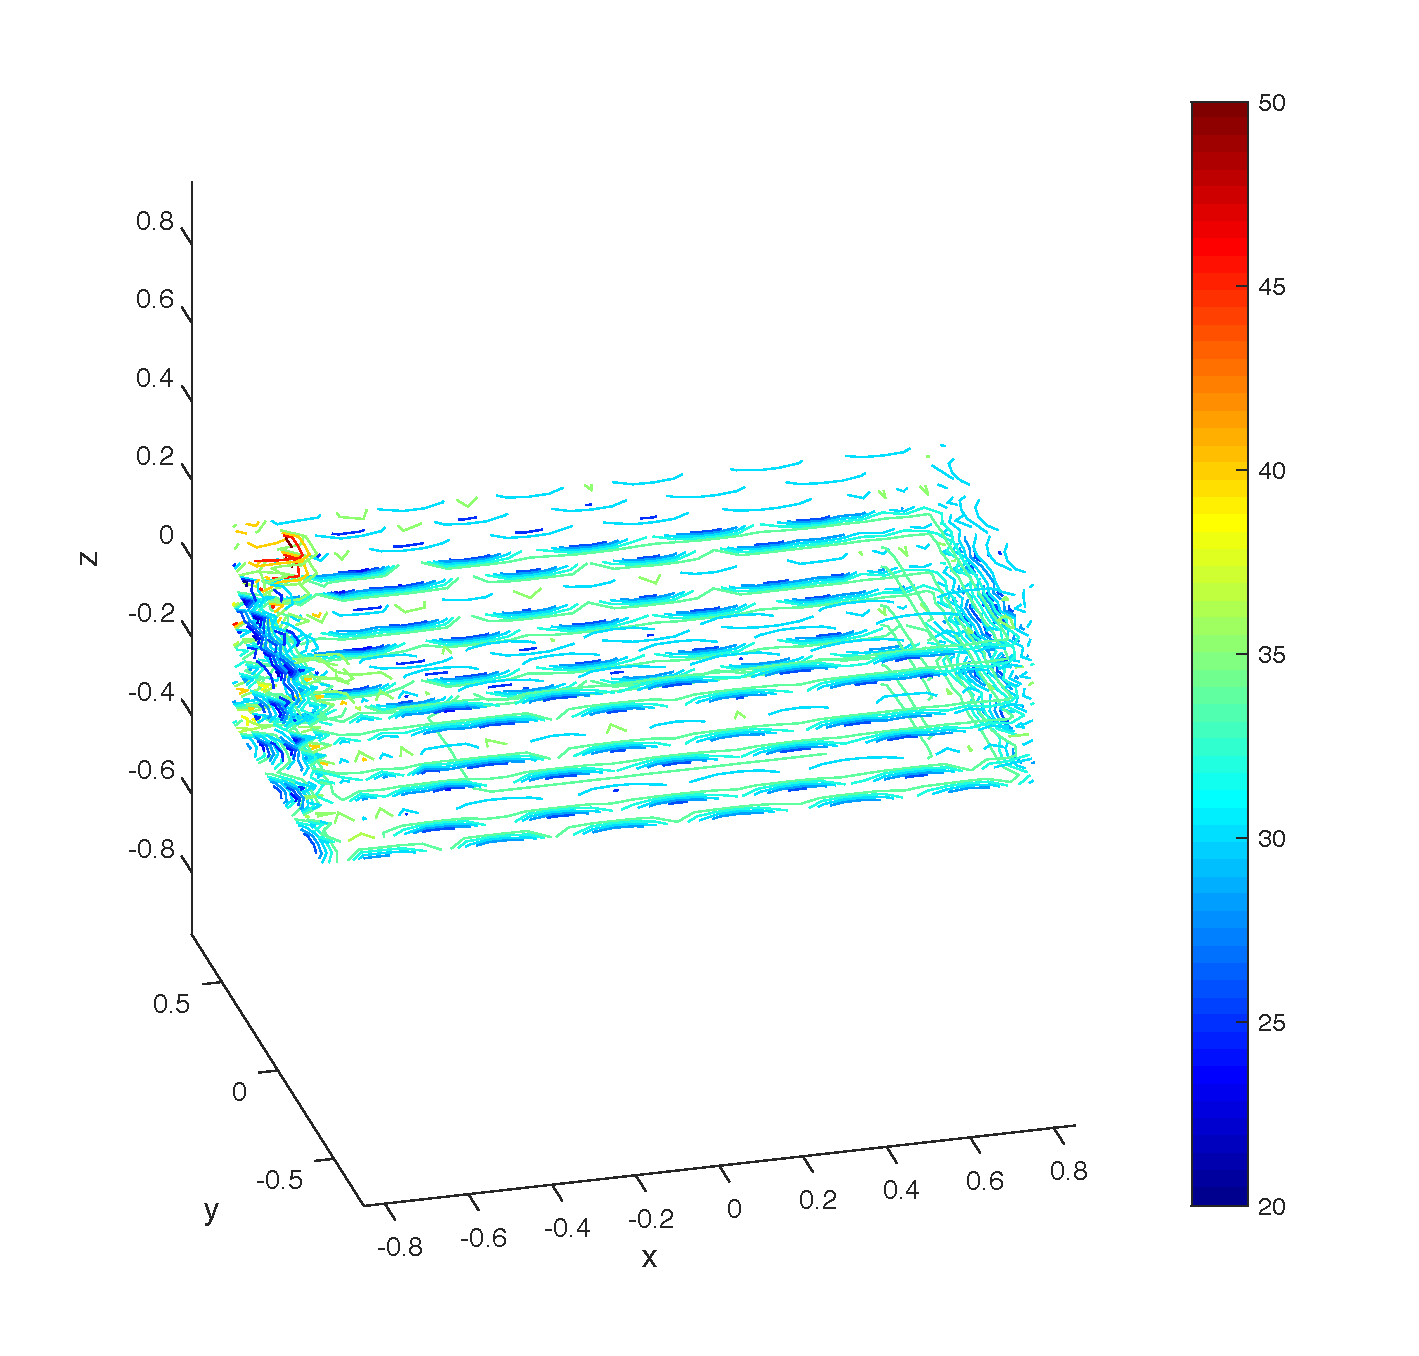
\includegraphics[width=8cm]{8-5.pdf}\\
  \caption{$u_h=30$,$v_h=0.2$,t=600}\label{8-5_p}
\end{figure}

\begin{figure}[htb]
  \centering
  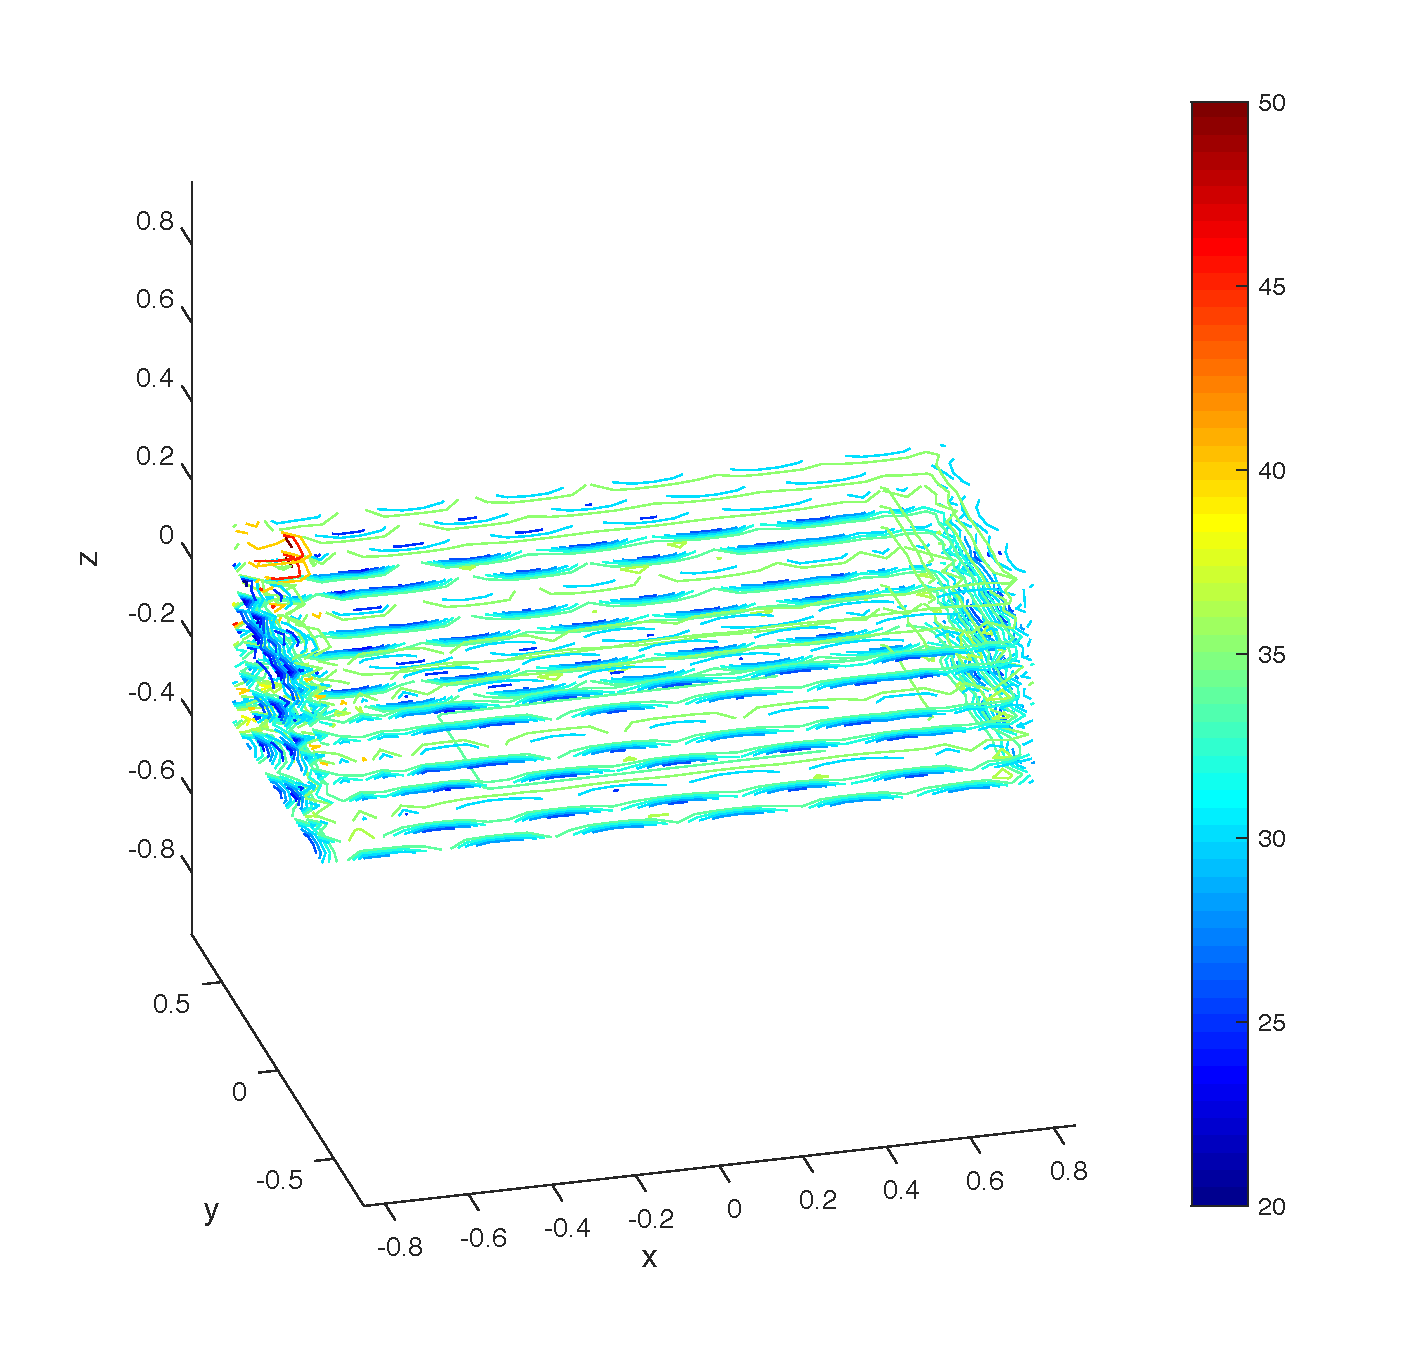
\includegraphics[width=8cm]{10-5.pdf}\\
  \caption{$u_h=40$,$v_h=0.2$,t=600}\label{10-5_p}
\end{figure}

\begin{figure}[htb]
  \centering
  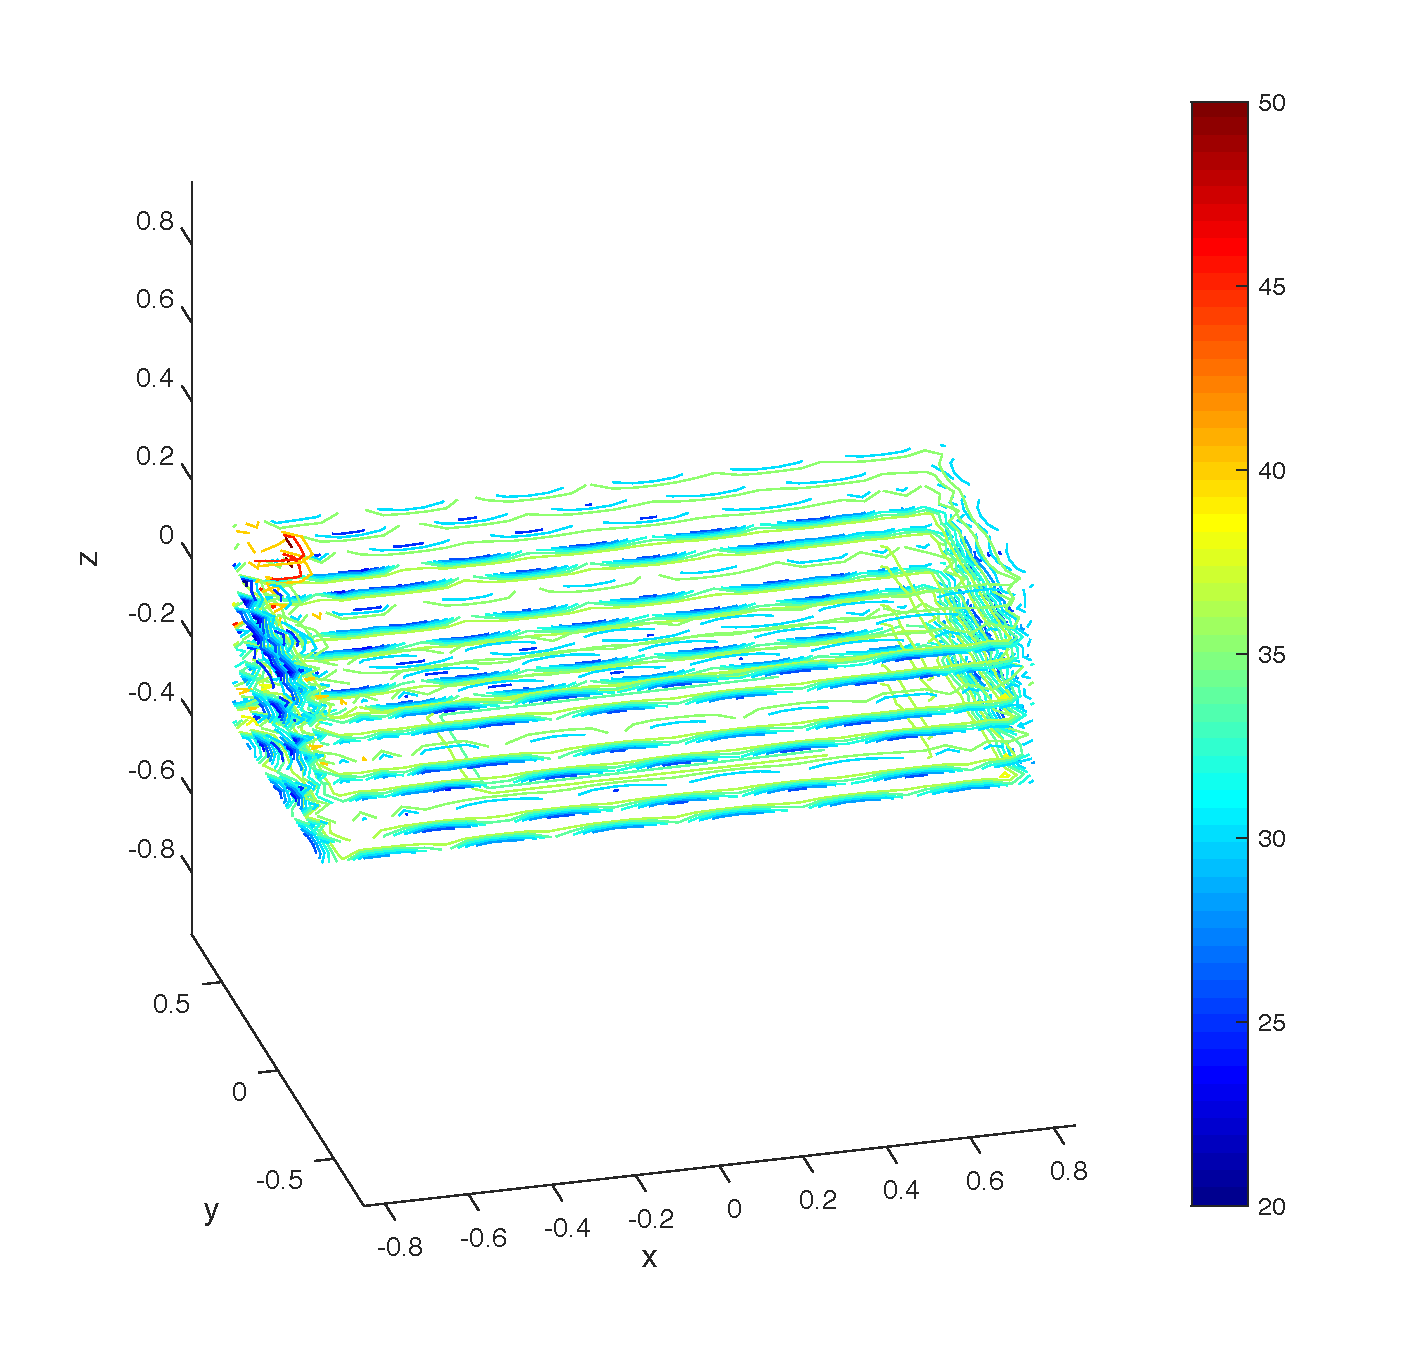
\includegraphics[width=8cm]{4-5.pdf}\\
  \caption{$u_h=50$,$v_h=0.2$,t=600}\label{4-5_p}
\end{figure}

It indicates that keep $v_h$, temperature increases when $u_h$ increases, and the system becomes more stable as time goes on. It proves that our model is sensible.

Comparing the temperature distribution of each strategy, with least water waste, we choose $v_h=0.2$, $u_h=40$ as the best strategy to keep the temperature.


\section{Sensitivity Analysis}
\label{sec:sensitivity-analysis}

\subsection{Parameters of Bathtub}
\label{sec:parameters of bathtub}
\begin{itemize}
\item We change the shape of the bathtub to sphere and cylinder to get the best strategy. The result shows that the bathtub with the shape of sphere is the most effective in keeping temperature.
\begin{center}
\begin{tabular}{c|c|c}
\hline
 Shape     &$v_h$  &$u_h$        \\ \hline
 Square    &0.2             & 40              \\ \hline
 Sphere    &0.15            & 40              \\ \hline
 Cylinder  &0.2             & 45              \\ \hline
\end{tabular}
\end{center}
     \item We change the volume of the bathtub without changing the proportion. The result in the following table shows that with the same $v_h$, $u_h$ increases as volume increases; with the same $u_h$, $v_h$ increases as volume increases.
\end{itemize}

\subsection{Parameters of Person}
\label{sec:parameters of person}
\begin{itemize}
\item Comparing the temperature graph with different shape of the person, we found when the shape gets more regular, $u_h$, $v_h$ decreases relatively.
\item Change the volume of the person. The result shows that, $u_h$, $v_h$ for best strategy increases when the volume increases.
\item Change the surface temperature of the person to get the best strategy. The result shows no noticeable change.
    \begin{center}
\begin{tabular}{c|c|c}
\hline
 Surface Temperature     &$v_h$  &$u_h$        \\ \hline
 $u_2=33.5$    &0.2             & 40              \\ \hline
 $u_2=33.5$    &0.15            & 40              \\ \hline
 $u_2=33.5$  &0.2             & 45              \\ \hline
\end{tabular}
\end{center}
\end{itemize}

\subsection{Effects of Motion}
\label{sec:effects of motion}
When the person in the bathtub makes motions, the heat exchange coefficient between the person and water ${\gamma}_2$ increases. That means heat exchange between water and the person increases. In another aspect, the air above flows, so that evaporation heat of water increases. Water loses more heat.

The effect is that more heat is called for to keep the temperature. So $u_h$ increases for best strategy to keep the temperature.

The effect is that more heat is needed to keep the temperature, consequently $u_h$ as the best strategy increases to keep the temperature.

\subsection{Effects of Bubble Bath Additive}
\label{sec:effects of bubble bath additive}
When bubble bath additive is added while initially filling the bathtub, bubbles stay on the surface and the evaporation of water to air is limited. So water loses less heat.

The effect is that less heat is needed to keep the temperature. So $u_h$ for best strategy decreases to keep the temperature.

\section{Strengths and Weaknesses}
\label{sec:strengths-and-weaknesses}

\subsection*{Strengths}
\label{sec:strengths}

\begin{itemize}
\item Our model make good use of thermology knowledge so it can reflect the situation in the real world realistically.
\item Our model build a 3D geometry to simulate the research object so it can show the exact situation.
\item Our model operates with different strategies and display the result by 3D geometry graph, so they could be compared in a visible way.
\item Our model proves the effect of time.
\end{itemize}

\subsection*{Weaknesses}
\label{sec:weaknesses}

\begin{itemize}
\item We assume that the water is still. In fact, streams flow and fluid dynamic is better taken into consideration. The actual situation is much complicated.
\item The model of the person should be more realistic. In fact, model of human body includes hands, legs or other parts, and the surface of human skin isn't even.
\item The condensation of water should be taken into consideration. Water that evaporate become water vapour, and some will condense into water on the bathtub.
\end{itemize}


% the reference
\begin{thebibliography}{99}


\bibitem{1} http://www.engineeringtoolbox.com

\bibitem{2} Umesh Gaur, Suk-fai Lau, Brent B. Wunderlich, and Bernhard Wunderlich, Heat Capacity and Other Thermodynamic Properties of Linear Macromolecules VI. Acrylic Polymers, J.Phys.Chem.Ref.Data, Vol.11, No4, 1982.

\bibitem{3} https://www.professionalplastics.com/professionalplastics/content/castacrylic.pdf

\bibitem{4} A. Khabari, M. Zenouzi, T. O’Connor and A. Rodas, Natural and Forced Convective Heat Transfer Analysis of Nanostructured Surface, Proceedings of the World Congress on Engineering 2014 Vol I, WCE 2014, July 2 - 4, 2014, London, U.K.

\bibitem{5} http://www.nzifst.org.nz/unitoperations/httrtheory3.htm

\bibitem{6} http://www.engineersedge.com/heat\_transfer/convective\_heat\_transfer\_coefficients\_\_13378.htm

\bibitem{7} de Dear. Richard J., Arens. Edward A, Zhang Hui and Oguro. Masayuki, Convective and radiative heat transfer coefficients for individual human body segments, Int J Biometeorol (1997) 40:141–156

\bibitem{8} http://www.hcheattransfer.com/coefficients.html

\end{thebibliography}

\label{LastPage}

\section{Non-technical explanation}

Users,

If you'd like to use the bathtub, it's better to acknowledge that:

\begin{itemize}
\item Obviously, the water exchange thermal energy directly with the air. That's why you can see water vapour float above the water. The temperature of water decreases as a result of the heat exchange.
\item On the other hand, the bathtub is cooler than the water on most occasions. It's reasonable that the bathtub absorbs heat from the water. However, the bathtub conduct heat easily, while in this way the air's temperature rises. In other words, the temperature of water decreases faster.
\end{itemize}
From statement above, you may understand our bathtub can't stay in an even temperature evenly. Consequently we have some suggestions for you, if you'd like to enjoy more during your bath :
\begin{itemize}
\item To keep the water warm and relax yourself, you may turn the faucet on. Water-in in high temperature loses it's energy quickly, and water-in in low temperature is unable to warm your surrounding. It's best that you set the speed of the water-in at 0.2kg/s, and temperature at $40\,^{\circ}\mathrm{C}$.
\item Further more, your movement effects the water. It would be great if you stay still, but it doesn't count too much. For a better temperature-keeping situation, you may add some bubble bath additive to decrease the temperature loss.
\end{itemize}
We hope you enjoy your bath.

\end{document}

%%% Local Variables:
%%% mode: latex
%%% TeX-master: t
%%% End:
